In Chapter~\ref{chap:problem-settings}, we posed the requirements that any solution must fulfil, in order to properly answer our research question. Then, in Chapter~\ref{chap:heaven}, we faced each requirement at design level, stating how an implementation of \name must be realised to fulfil them. 

In this chapter, we describe the implementation experience of \namens: 
Firstly in Section~\ref{sec:test-stand-general}, we present the pillar concepts of this development: the basis abstractions, in Section~\ref{sec:abstractions}, and the data model of the \textsc{Test Stand}, in Section~\ref{sec:data-impl}. In Section~\ref{sec:modules-impl}, we introduce each \name module: the \textsc{Streamer}, the \textsc{ResultCollector} and the \textsc{Test Stand Supporting Structure}. In Section~\ref{sec:baselines-impl}, we present how we implement the four baseline RSP Engines. Finally, in Section~\ref{sec:analyser-impl}, we describe how the \textsc{Analyser} Investigation Stack is realised w.r.t the Evaluation we will present in Chapter~\ref{chap:evaluation}.

\section{Test Stand}\label{sec:test-stand-general}

The architecture of the \textsc{Test Stand} consists of three stand alone modules that establish a mono-directional communication flow: the \textsc{Streamer}, the \textsc{RSP Engine} and the \textsc{Result Collector}. Moreover, the idea of an external structure which supports the other modules brings to the concept of the \textsc{Test Stand Supporting Structure}. All these components communicate exchanging events data, exploiting an event-based and modular architecture as demanded by [R.10] and [R.11]. In the following, we presents the two abstractions that allow this architecture: \textit{EventProcessor} and the \textit{Event}. Then, we detail how the \textsc{Test Stand} Data Model is implemented.

\subsection{Abstractions}\label{sec:abstractions}

Among all the requirements reported in Section~\ref{sec:requirements}, two of them are immediately relevant: [R.10], i.e. the need of an \textit{Extendible Design}, and [R.11], which states the necessity of an \textit{Event-base architecture} to properly face any RSPEngine. In order to to fulfil both, the \textsc{Test Stand} requires two main abstractions:
\begin{itemize}
\item The \textit{Event} - which is required to build a hierarchical communication. Indeed, the \textsc{Test Stand} may handle three event flows: one internal to the RSP Engine module, one for the communication between modules and one to communicate with the user. Next section about data clarifies the communication structured. 
\item The \textit{Event Processor} -  guarantees the system to be modular and it standardizes the interaction simplifying the behaviour of each component in the system. Thus, a module is an \textit{Event Processor} which can be positioned everywhere in the the \textsc{Test Stand} pipeline.
\end{itemize}

\begin{figure}[h!tb]
  \centering
	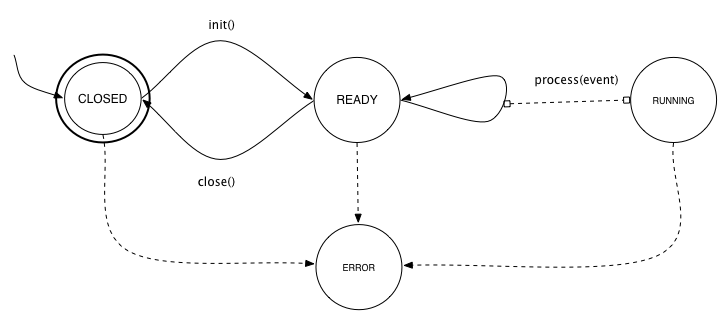
\includegraphics[width=\linewidth]{images/fsm-schema}
	\caption[\textit{EventProcessor} States Diagram]{The finite state machine diagram of any \name module and the Baselines. It is realised through the \textit{Startable} interfaces, which provide the \textit{init()} and \textit{close() }methods, and through the \textit{EventProcessor} interface, which declares the \textit{process(Event e)} method. The execution is possible only during the RUNNING state, which can be achieved by one and only module at time, as a constrain. The ERROR state prevents the propagation of erroneous behaviour to the data.}
  	\label{fig:module-fsm}
\end{figure}

\noindent The requirement [R.4] directly influences the  the \textsc{Test Stand} workflow stating that it must not be running when the RSP Engine is under execution. To cover this requirement, we designed each module as a Finite State Machine (FSM), which can work only specific states that allow processing (READY). 

Each \name module, the Baselines, and also for the \textsc{Test Stand External Structure} follows the FSM in Figure~\ref{fig:module-fsm}, implemented through two interfaces: 

The \textit{Startable} interface standardises two methods, \textit{init()} and \textit{close()} which allow to control the behaviour of the module at the beginning and the end of the execution. The interface allows to move from the CLOSED state to the READY through the \textit{init()} method and from the READY to the CLOSED through the \textit{close()} method. 

\textit{EventProcessor} interface completes the FSM schema, exposing the \textit{process (Event e)} method. The method brings the module into the RUNNING state until the processing ends, and then back to the READY one. As a constrain, one and only one module can be in the RUNNING state in a certain moment during the execution.

Finally, the ERROR State, which can be reached from any point of the execution, prevents the propagation of errors over result data: when a module fails the execution is stopped without saving the erroneous data (last event) and reporting the error to the user.\\


\noindent [R.4] is fulfilled because each module in the systems fulfils [R.10] and [R.11]. \name Modules can be explicitly controlled by the \textsc{Test Stand Supporting Structure}, which starts and stops the processing through the methods exposed by the \textit{Startable} and \textit{EventProcessor} interfaces. It bring the modules from one status to another one, according with the FSM schema in Figure~\ref{fig:module-fsm}.

\pagebreak

\subsection{Data Model}\label{sec:data-impl}

In the previous sections, we stated that the \textsc{Test Stand} and its modules exploit an event-based communication, as required by [R.11]. Chapter~\ref{chap:heaven} describes \name workflow and how it exchanges events during the execution. Each event represents different data, depending on its position in the workflow. The \textit{Event} concept we introduced, which is implemented as an interface, allows to give a hierarchy to the exchanged events. In general, the Test Stand handles four kinds of event, which are reported in Figure~\ref{fig:uml_events} and defined as follow:

\begin{figure}[h!tb]
  \centering
	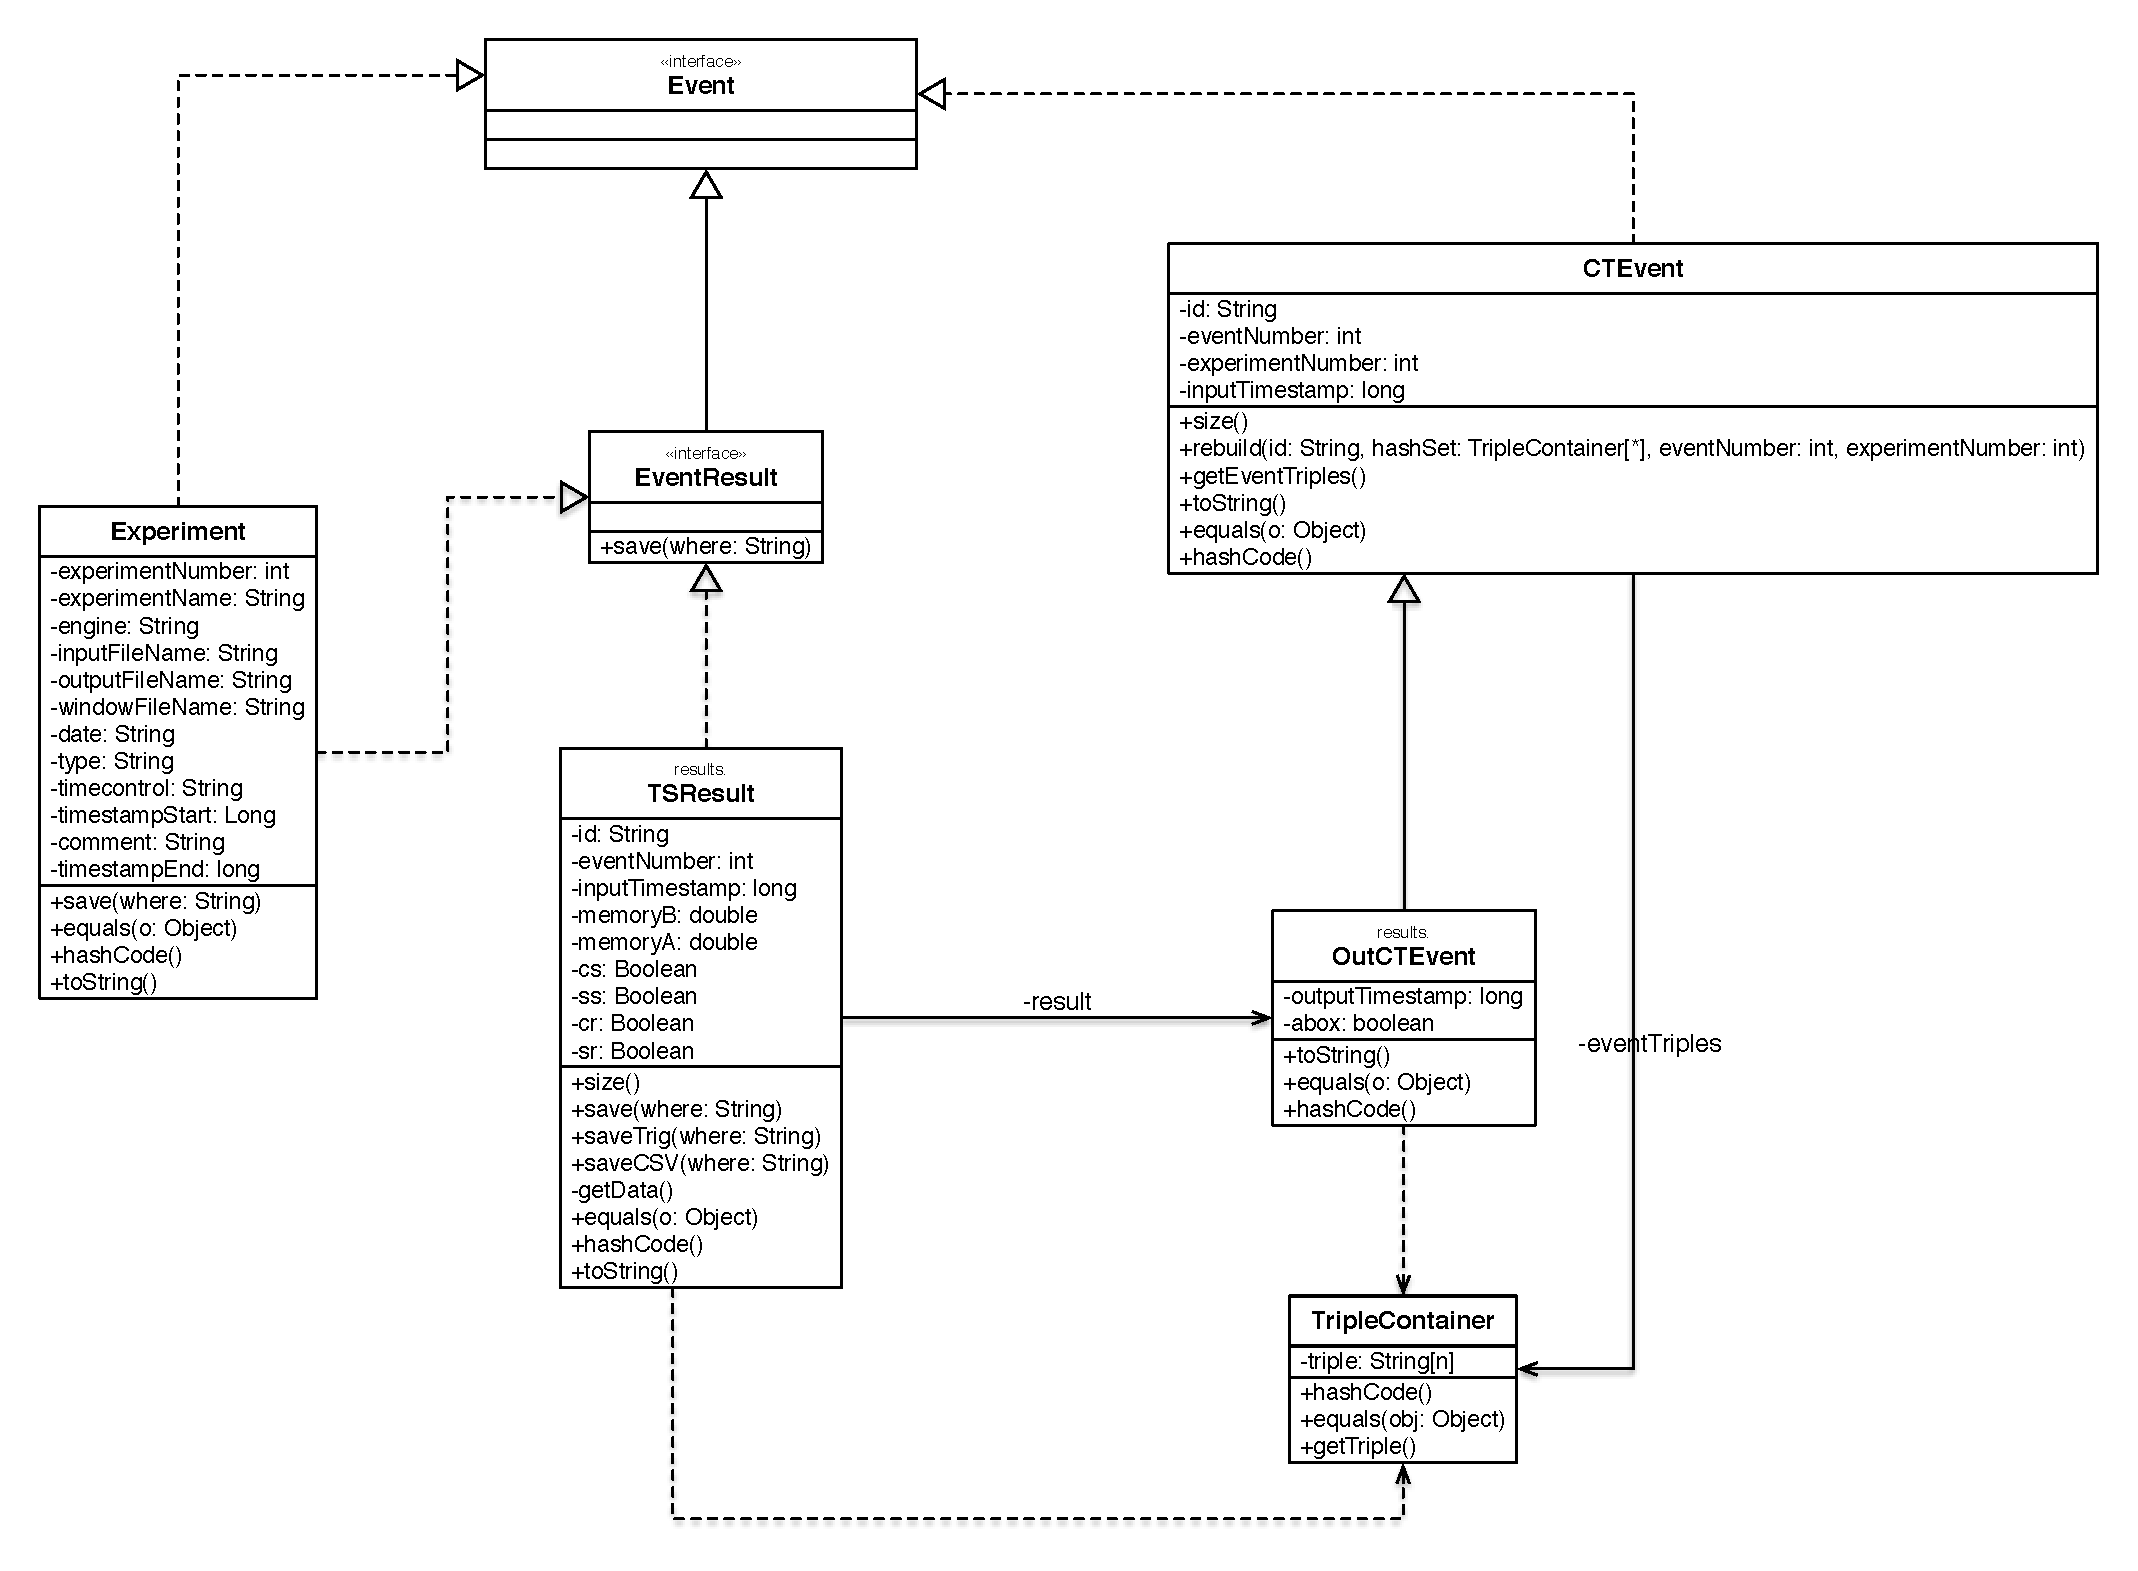
\includegraphics[width=\linewidth]{images/uml_events}
	\caption[\name Execution Events - UML Schema]{The figure shows the events that \name \textsc{Test Stand} and its modules 	exchange during the execution of an experiment. All of them implement the \textit{Event} interfaces that is at the top of the class 	hierarchy.} 
	\label{fig:uml_events}
\end{figure}

\begin{itemize}
\item \textit{Experiment} - it represents the tuple $<\mathcal{E}, \mathcal{D},\mathcal{T},\mathcal{Q}>$, indicating which RSP~Engine ($\mathcal{E}$) will be tested and with which queries ($\mathcal{Q}$), data ($\mathcal{D}$) and ontology  ($\mathcal{T}$) will be used. It contains the execution start time and the end time. A specific field indicates if the current implementation of the engine exploit external timing, while the $type$ parameter indicates which kind of testing will be applied (SOAK o Stress for example).
\item \textit{CTEvent} - it contains a set of contemporary triples, wrapped in the \textit{TripleContainer}. The id field identifies is unique for the event within the experiment.
\item \textit{OutCTEvent} - it represents the event produced by the RSPEngine after processing the active window. Figure~\ref{fig:uml_events} shows the inheritance relation with \textit{CTEvent}:  \textit{OutCTEvent} extends the \textit{CTEvent} adding the outputTimestamp field.
\item \textit{TSResult} - it wraps the \textit{OutCTEvent} adding the information about the measurements data gathered during the execution: memory, sampled ante e post processing, and latency. Two boolean fields allow to mark complete and soundness result, if it is evaluated at runtime (see Section~\ref{sec:requirements})
\end{itemize}

\name requires an initialization phase to prepare and input the \textit{Experiment} into the \textsc{Test Stand}. The current implementation exploits a property file with the Experiment parameters: ID and the tuple $<\mathcal{E}, \mathcal{D},\mathcal{T},\mathcal{Q}>$. 

The \textit{CTEvent} and the \textit{OutCTEvent} contain RDF triples in NT-Triple\footnote{http://www.w3.org/2001/sw/RDFCore/ntriples/}, which is the easiest RDF serialisation to parse. This serialisation was chosen to fulfil requirement [R.12], which demands an \textit{Easy-to-Parse RDF Serialisation for the events presented to the RSP Engine in exam}. Figure~\ref{fig:uml_events} shows also that the RDF Triples are stored in the events into the \textit{TripleContainer} wrapper: we redefine the triple hashcode and equals method guaranteeing their uniqueness within an \textit{CTEvent} or \textit{OutCTEvent}.

\section{Test Stand - Modules}\label{sec:modules-impl}

In this section we present the two of modules which compose \namens, the \textsc{Streamer}, in Section~\ref{sec:streamer-impl} and the \textsc{ResultCollector} in Section~\ref{sec:result-collector-impl}, while the \textsc{RSPEngine} will be introduced in Section~\ref{sec:baselines-impl}. Moreover, in Section~\ref{sec:teststand-impl} we details the \textsc{Test Stand Supporting Structure}. %They all extend the \textit{EventProcessor} and the \textit{Startable} interfaces as reported in Section~\ref{sec:abstractions}.

In Section~\ref{sec:abstractions}, we define a module as an \textit{EventProcessor} which can be positioned everywhere in the the \textsc{Test Stand} pipeline. We state that a module must implements the \textit{Startable} interface, which completes the FSM schema in Figure~\ref{fig:module-fsm} with the \textit{init()} and \textit{close()} methods.

\subsection{Streamer}	\label{sec:streamer-impl}

\begin{figure}[tbh]
  \centering
	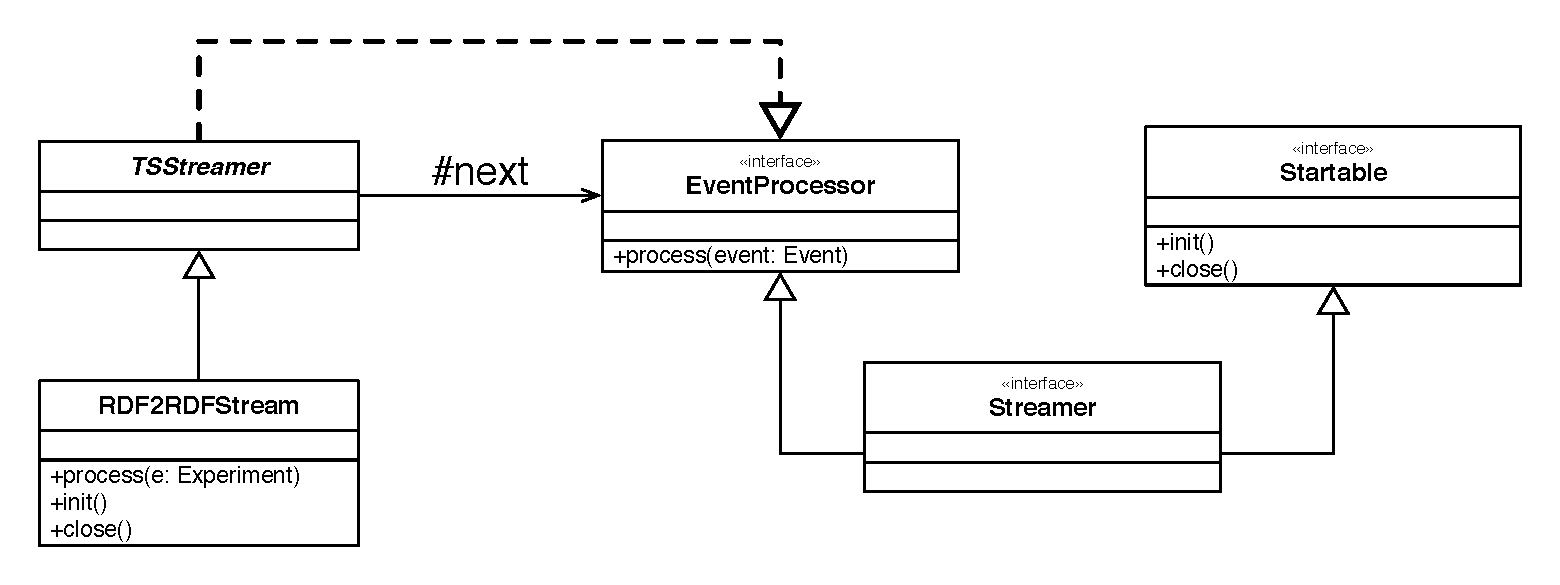
\includegraphics[width=\linewidth]{images/uml_tstreamer}
	\caption[\textit{RDF2RDFStream \textsc{Streamer} Implementation} - UML Schema]{\textit{RDF2RDFStream} \textsc{Streamer} Implementation. The \textit{RDF2RDFStream} extends the \textit{TSStreamer} abstract class, which defines the module as a \textit{Startable} \textit{EventProcessor} of \textit{Experiment}s} 
  	\label{fig:uml_tstreamer}
\end{figure}

\noindent Figure~\ref{fig:uml_tstreamer} shows the current implementation of the \textit{Streamer} interface, which is the head of  the \textsc{Test Stand} pipeline. Actually, the \textit{Streamer} is implemented as the \textit{TSStreamer} abstract class, which is specialised into processing of \textit{Experiment} events. 

The \textit{Experiment} events are  externally instantiated and then \textit{TSStreamer} receives them. It can start the processing only if it is initialised. It communicates with another \textit{EventProcessor}, called \textit{next}, which can receive  \textit{CTEvent}s. In Figure~\ref{fig:uml_tstreamer} the \textit{next} is represented by the labelled arrow.  Notice that, also the \textit{next} must be initialised before starting the communication, otherwise the ERROR state will be reached, since the processing is not allowed.

\noindent Figure~\ref{fig:uml_tstreamer} contains also the \textit{RDF2RDFStream} implementation, whose internal structure can be seen in Figure~\ref{fig:uml_flowrateprofiler}. The \textit{RDF2RDFStream} was developed to conduct experiments as they are presented in Chapter~\ref{chap:evaluation}.  We use the LUBM Benchmark to generate the data for the experiments, but it actually generates static data and, thus, we translate them to a streaming scenario through the \textit{RDF2RDFStream}, which builds an RDF Stream attaching a timestamp to the static data produced by LUBM. %The file is generated using  LUBM(1000,0), which means 1000 different universities with the random generation seed 0. 

\begin{figure}[tbh]
  \centering
	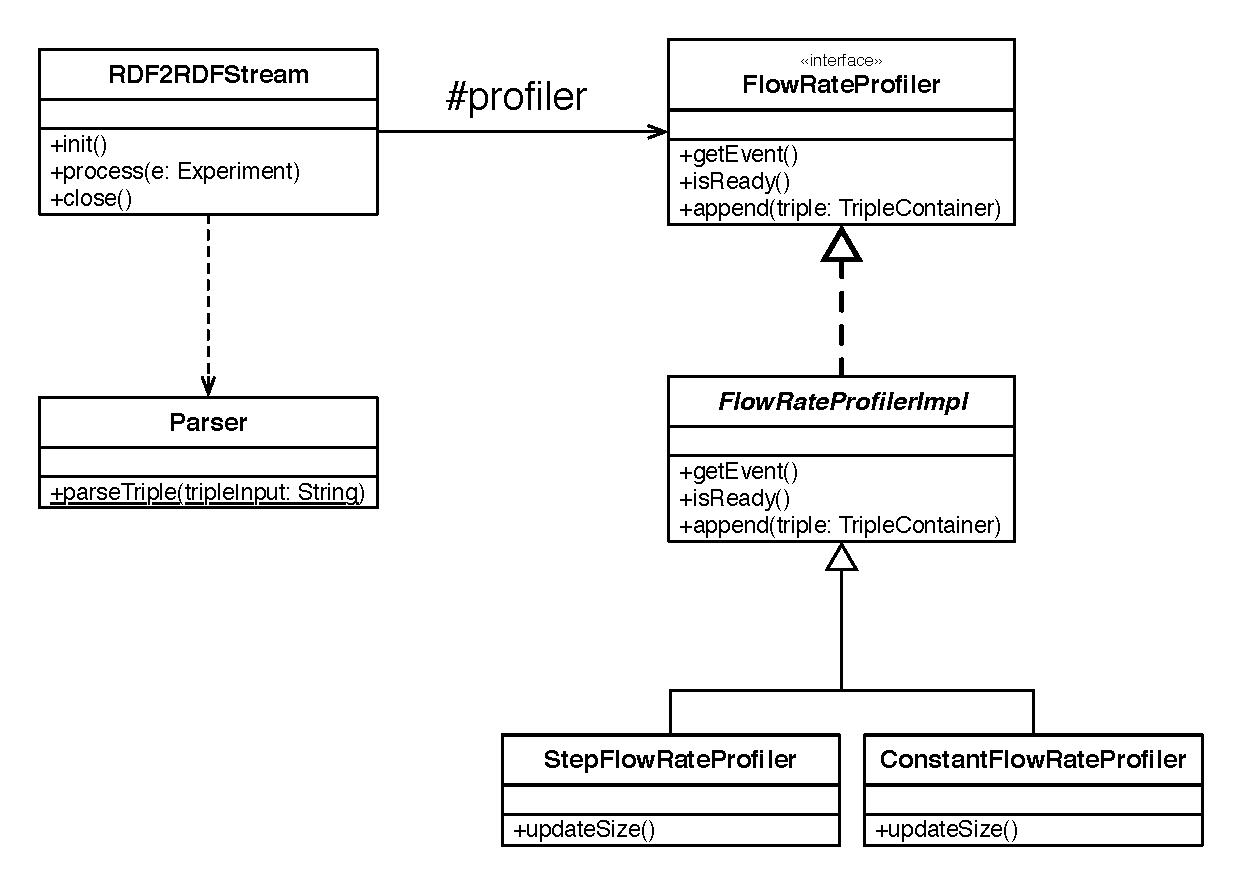
\includegraphics[width=0.75\linewidth]{images/uml_flowrateprofiler}
	\caption[Internal Components of \textit{RDF2RDFStream} - UML Schema]{The \textit{RDF2RDFStream} exploits two subcomponents to build an RDF Stream: the \textit{Parser}, which allows to read in memory RDF Triples, and the \textit{FlowRateProfiler}, which attaches to RDF triple a timestamp and it builds \textit{CTEvent}s according to a function $f$. The \textit{FlowRateProfileImpl} provides implementation of the \textit{append(TripleContainer tc}) method and of the two utility methods \textit{isReady()} and \textit{getEvent()}. Specific implementations of the \textit{FlowRateProfiler} control the function $f$ through the \textit{updateSize()} method.} 
  	\label{fig:uml_flowrateprofiler}
\end{figure}


The \textit{Parser} component, in Figure~\ref{fig:uml_flowrateprofiler}, can be accessed statically. It reads in memory, one by one the triples, in the file, guaranteeing data independence [R.1] and it does not influence the memory footprint [R.5], because it allocates only the memory necessary to parse a triple. 

Figure~\ref{fig:uml_flowrateprofiler} also includes the \textit{FlowRateProfiler}. This component determines the number of triples to add to a \textit{CTEvent} and it builds such an event. In this way, \textit{RDF2RDFStream} can generate many RDF~Streams to use as $\mathcal{D}$, which differ on the number of contemporary triples. 

\begin{figure}[tbh]
\centering
\subfigure[Exponential Growing \textsc{CTEvent} Size: $y=2^x$]{
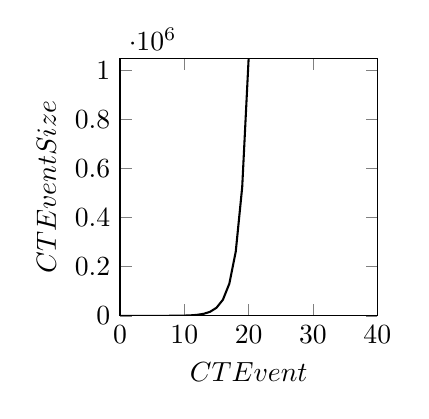
\begin{tikzpicture}
  \begin{axis}[ 
  width=0.4\linewidth,
      height=0.4\textwidth,
    xlabel=$CTEvent$,
    ylabel={$CTEvent Size$},
    xmin=0.00, xmax=40,
	ymin=0, ymax=1048576
  ] 
    \addplot [
    line width=0.75pt]
    coordinates {
    		(0.00, 1.00)
		(1.00, 2.00)
		(2.00, 4.00)
		(3.00, 8.00)
		(4.00, 16.00)
		(5.00, 32.00)
		(6.00, 64.00)
		(7.00, 128.00)
		(8.00, 256.00)
		(9.00, 512.00)
		(10.00, 1024.00)
		(11.00, 2048.00)
		(12.00, 4096.00)
		(13.00, 8192.00)
		(14.00, 16384.00)
		(15.00, 32768.00)
		(16.00, 65536.00)
		(17.00, 131072.00)
		(18.00, 262144.00)
		(19.00, 524288.00)
		(20.00, 1048576.00)
		};	
		
	\end{axis}
\normalsize

\end{tikzpicture}
}
\subfigure[Step Growing Size with K1=100 and K2=1000 after 9 \textsc{CTEvents}]{
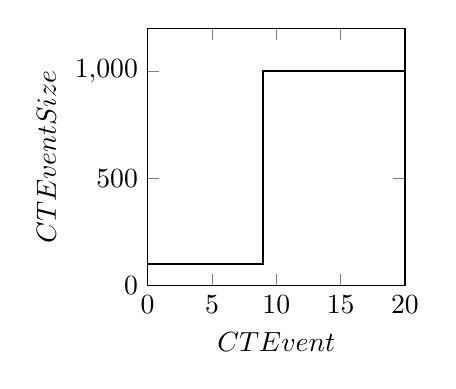
\begin{tikzpicture}
  \begin{axis}[ 
  width=0.4\linewidth,
      height=0.4\textwidth,
    xlabel=$CTEvent$,
    ylabel={$CTEvent Size$},
    xmin=0.00, xmax=20,
	ymin=0, ymax=1200
  ] 
    \addplot [
    line width=0.75pt]
    coordinates {
    		(0.00, 100.00)
		(1.00, 100.00)
		(2.00, 100.00)
		(3.00, 100.00)
		(4.00, 100.00)
		(5.00, 100.00)
		(6.00, 100.00)
		(7.00, 100.00)
		(8.00, 100.00)
		(9.00, 100.00)
		(9.00, 1000.00)
		(10.00, 1000.00)
		(11.00, 1000.00)
		(12.00, 1000.00)
		(13.00, 1000.00)
		(14.00, 1000.00)
		(15.00, 1000.00)
		(16.00, 1000.00)
		(17.00, 1000.00)
		(18.00, 1000.00)
		(19.00, 1000.00)
		(20.00, 1000.00)
		};	
		
	\end{axis}
\normalsize

\end{tikzpicture}
}
\caption[Example of FlowRateProfiler Triple Distribution]{The \textsc{FlowRateProfiler} is able to calculate \textsc{CTEvent} size according to a function which relates the number of triple to the number of \textsc{CTEvent} }
\label{fig:frp-examples}
\end{figure}


The \textit{FlowRateProfilerImpl} implements \textit{FlowRateProfiler} interface. It provides a common implementation for the method \textit{append(TripleContainer tc)}, which adds to the current \textit{CTEvent} an RDF triple,  and of the two utility methods \textit{isReady()} and \textit{getEvent()}. What variates between different implementations of this component, is the \textit{updateSize()} method. 

The \textit{FlowRateProfiler} creates \textit{CTEvent} according to a function $y=f(x)$, in which $x$ is the \textit{CTEvent} id and it results that $y$ is the number of triple this \textit{CTEvent} will contain.  $f$ is implemented within the \textit{updateSize()} method. For example if we decide to increase linearly the number of triples inside a \textit{CTEvent} the function $f$ will be: \[y=x, \text{ where } x,y \in N\]
The first event (E0) will contain zero triple, E1 will contain only one triple, E4 will contain four triples and so forth. Another possibility is to increase exponentially the number of triples inside a \textit{CTEvent} : \[y=2^x, \text{ where } x,y \in N\]The first event (E0) will contain one triple, E1 will contain two triple, E3 will contain eight triples and so forth. Figure~\ref{fig:frp-examples}.a shows the resulting behaviour plotting the triple number on y-axis and \textit{CTEvent} id on x-axis.

In the current stage of development, we include four implementations of the \textit{FlowRateProfiler}, two of them are related to our experiments: 
\begin{itemize}
\item \textit{ConstantFlowRateProfiler} - it maintains the same number of triples for each event over all the experiment: \\
\[y=K, \text{ where } K \in N \]

\item \textit{StepFlowRateProfiler} - it maintains a constant number of triple $K1$ inside a \textit{CTEvent} for $x$ occurrences, then it suddenly changes the number of triple $y$ form $K1$ to $K2$ where $K2 >> K1$. The number of  \textit{CTEvents} $x$ is specified in the set-up phase of the component.  Figure~\ref{fig:frp-examples}.b contains the resulting plot of implemented function which follows:

\[
y=
\begin{cases}
K1, &\text{if $x < M$ } $ where $ K1, M \in N\\
K2, &\text{if $x >= M$} $ where $ K2 >> K1, K2 \in N
\end{cases}
\]


\end{itemize}

The remaining two  \textit{FlowRateProfiler} implementations in \name that are not related to our evaluation are:
\begin{itemize}
\item \textit{LinearStepFlowRateProfile} - it streams $x$ \textsc{CTEvents} of dimension $y$, in terms of triples, then linearly increase the number of a quantity $M$: \[y=x*M, \text{ where } x,y,M \in N\]
%\item \textit{ConstantRandomFlowRateProfiler} - it changes $y$ and $x$ according with two random integer generators directed by two seeds. The generators provided integer numbers according to a certain probability \[y=randomInt(seed), \text{ where } random(seed),y \in N\]
\item \textit{PoissonFlowRateProfiler} - it changes $y$ and $x$ according with a parameter $\lambda$, which indicates the Expected Value of a Poisson Distribution that is

\[y=e^{- \lambda \frac{\lambda^n}{n}}, \text{ where } n \in N  \]
\end{itemize}


\subsection{Result Collector}\label{sec:result-collector-impl}

\noindent The \textsc{ResultCollector} is the data acquisition system that receives and persists the query results and the measurements data gathered by the \textsc{Test Stand} during the execution of an experiment.

\begin{figure}[tbh]
  \centering
	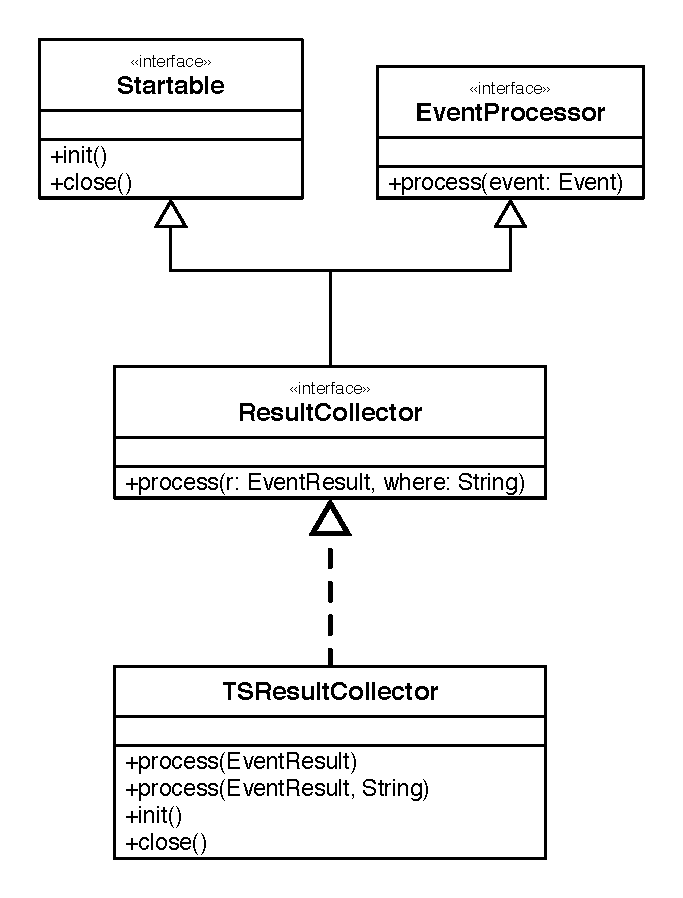
\includegraphics[width=0.5\linewidth]{images/uml_resultcollector}
	\caption[\textsc{ResultCollector} Current Implementation - UML Schema]{The current implementation of the \textsc{ResultCollector} interface is the \textit{TSResultCollector} which processes events that implement the \textit{EventResult Interface}. \textit{ResultEvent} interface hides the saving procedure, delegating the implementation to the event provider through    the \textit{save()} method. \textit{TSResultCollector} exposes also the method \textit{process(Event e, String where)}, which allows the caller to specify the destination. } 
  	\label{fig:uml_resultcollector}
\end{figure}

The UML Schema, in Figure~\ref{fig:uml_resultcollector}, shows the \textit{ResultCollector} interface, another proxy for the \textit{EventProcessor} and the \textit{Startable} ones. The current implementation is the \textit{TSResultCollector}, which stays at the end of the \textsc{Test Stand} pipeline. The \textit{ResultCollector} is responsible of saving data independently from their format, since requirement [R.7] demands to \textit{enable users extensions to the basic measurement set}. The \textit{TSResultCollector} applies a general saving procedure exploiting the \textit{EventResult} interface, which exposes the \textit{save(String where)} method, delegating the implementation of such procedure to the provider of the event. Figure~\ref{fig:uml_resultcollector} shows the relation between the \textit{EventResult} interface and the \textit{TSResultCollector}, which specialises the processing method to \textit{process(EventResult)} and it knowns the general destination of the data, but it also exposes a secondary one \textit{process(EventResult er, String where)}, which allows the caller to specify the saving path.


\begin{figure}[tbh]
  \centering
	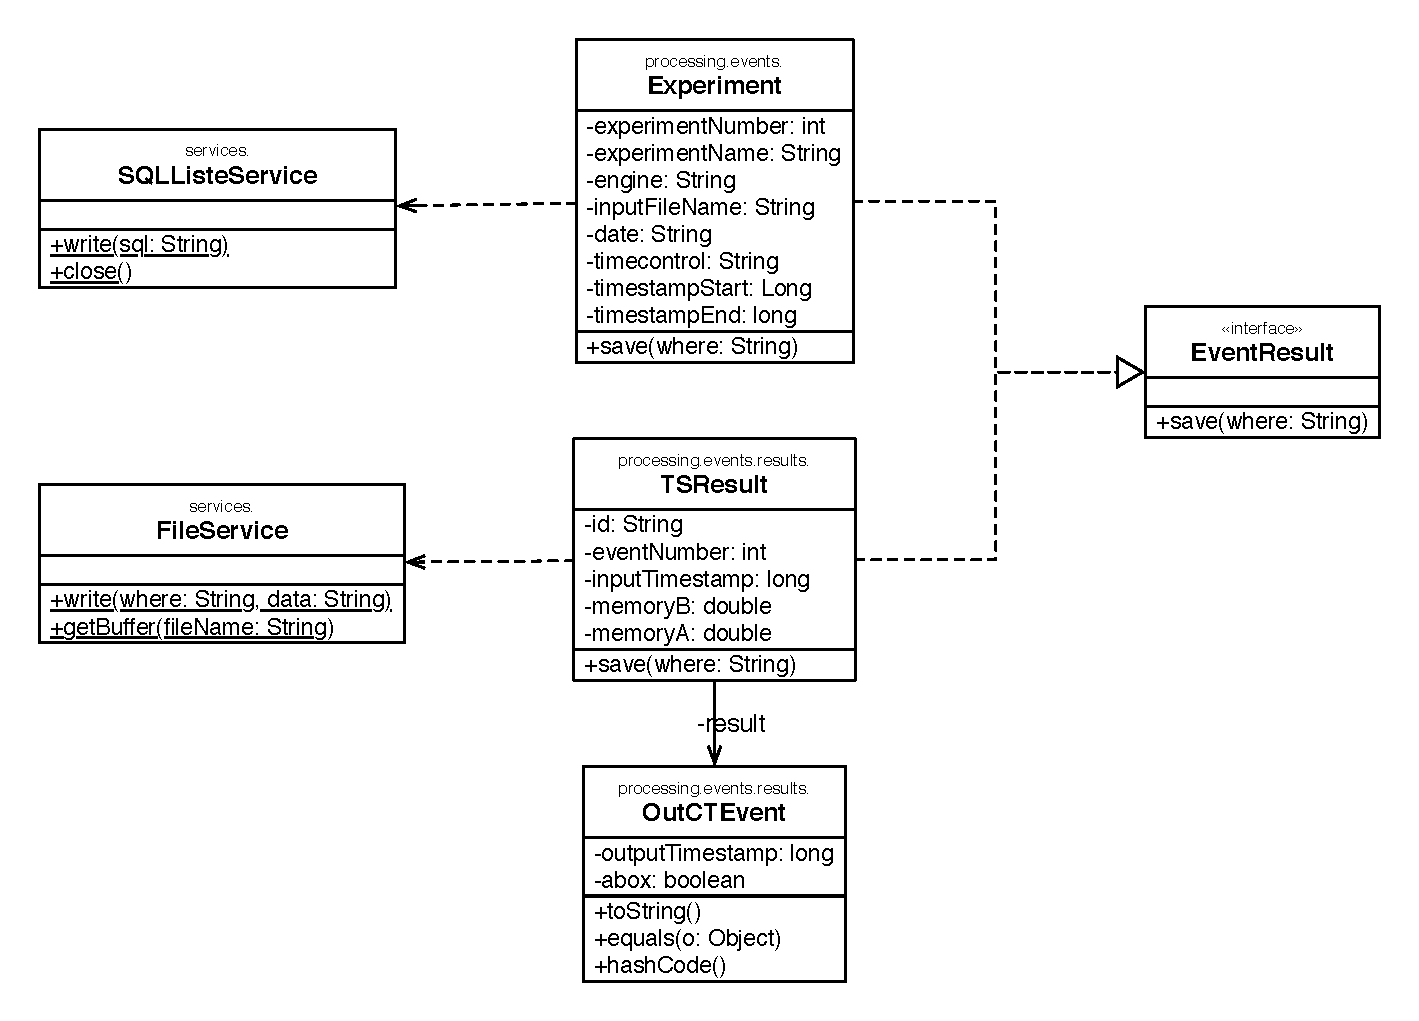
\includegraphics[width=\linewidth]{images/uml_resultcollector_events}
	\caption[\textsc{ResultCollector} Events - UML Schema]{The \textit{Experiment}, the \textit{TSResult} and the \textit{OutCTEvent} implement the \textit{EventResult} interface, hiding the saving procedure through the \textit{save(String where)} method. In the current implementation, they exploit the \textit{FileService} and the \textit{SQLLIsteService} classes, to avoid concurrent accesses to the file system.} 
  	\label{fig:uml_resultcollector_events}
\end{figure}

\pagebreak

\noindent Figure~\ref{fig:uml_resultcollector_events} shows which events in the system exploit the \textit{EventResult} interface. In the current implementation, the \textit{TSResultCollector} handles two kinds of event:
\begin{itemize}
\item \textit{TSResult} - it saves the data of the query results into a TriG\footnote{http://www.w3.org/TR/trig/} file where the graph name is the event id inside the experiment, while it saves the measurements data into a CSV\footnote{$http://en.wikipedia.org/wiki/Comma-separated_values$} file that represents the time series w.r.t events id. 
\item \textit{Experiment} - it saves the experiment metadata and the tuple \\ $<\mathcal{E},\mathcal{D},\mathcal{T},\mathcal{Q}>$ collapsed into a generic description field into SQLite\footnote{https://sqlite.org/} database.
\end{itemize} 

Both saving procedures exploit a service class, respectively the \textit{FileService} and the \textit{SQLLIsteService}. In Figure~\ref{fig:uml_resultcollector_events}, we describe such services, which expose static methods to interact with the file-system. The goal is reduce system complexity and avoid parallel interactions that may influence the experiment, offering a single point to interact with the file-system. 


\subsection{Test Stand Supporting Structure}\label{sec:teststand-impl}


\begin{figure}[tbh]
  \centering
	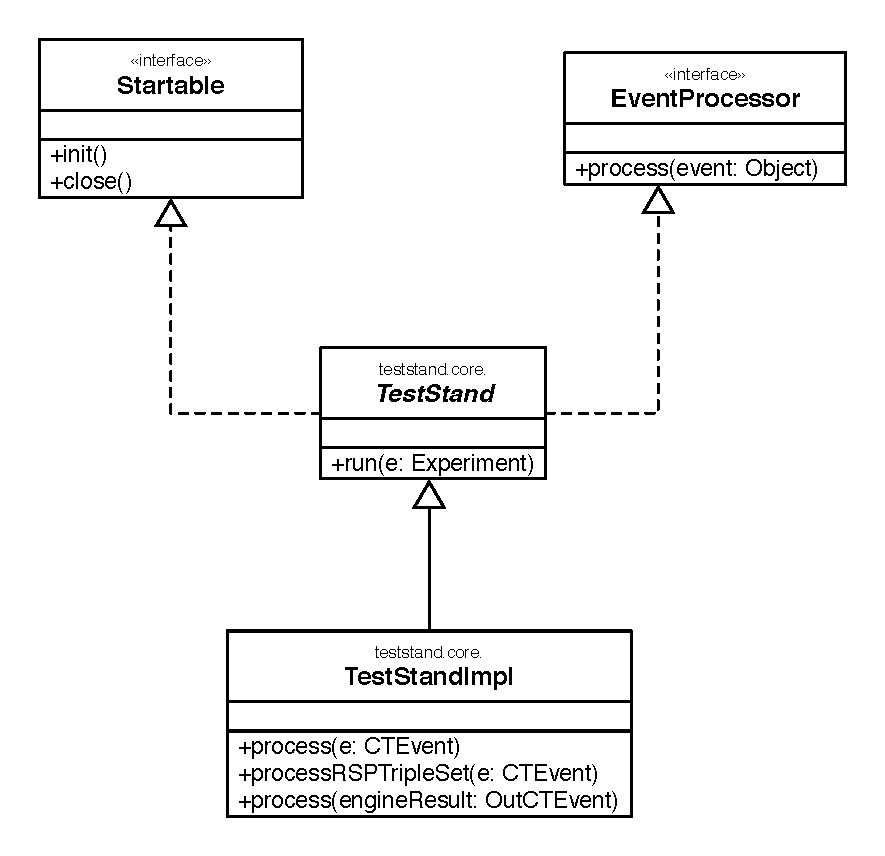
\includegraphics[width=0.5\linewidth]{images/uml_teststand}
	\caption[\name \textsc{TestStand} - UML Schema]{The \textit{EventProcessor} and the \textit{Startable} method are implemented in two class levels: the \textit{init()} and \textit{close()} methods depend on the \textit{TestStand} abstract class, while the  \textit{process(CTEvent e)} method is implemented by \textit{TestStandImpl} class, which represents the \textsc{Test Stand Supporting Structure}. Moreover, it exposes also the \textit{run(Experiment e)} method to start the processing.}
  	\label{fig:uml_teststand}
\end{figure}


\noindent \name \textsc{Test Stand} was defined as set of modules which interact exchanging events during the execution. However, Chapter~\ref{chap:heaven} describes at the design level the presence of an supporting structure which orchestrates the communication between the \textsc{Streamer}, the \textsc{RSP Engine} and the \textsc{ResultCollector}. This supporting structure also exposes the APIs for users interaction. Figure~\ref{fig:uml_teststand} represents this idea into an UML schema where the abstract class \textit{TestStand} implements both the \textit{Startable} interface, defining the \textit{init()} and \textit{close()} methods and also the \textit{EventProcessor} interface, however it leaves the implementation of the \textit{process(CTEvent e)} method to the current implementation: the \textit{TestStandImpl}. 

The relation between the \textit{TestStand} and other modules is presented in Figure~\ref{fig:uml_teststand_modules}. The \textit{TSStreamer}, the \textit{RSPEngine} and the \textit{TSResulCollector} are linked to the \textit{TestStandImpl} through an initialisation class which receives the configuration file, and sets up these modules according with the requirements [R.1]  [R.2] and [R.3] (respectively data independence, engine independence and query independence). Once the set-up phase is completed, the \textit{TestStandImpl} is initialized and it consequently initialises all the upstanding modules. The \textit{Experiment} is created externally and  the \textit{TestStandImpl} receives it to start the execution. 

During the execution, \textit{TestStandImpl} gets the \textit{CTEvents} from the \textit{TSStreamer} and it sends them to the \textit{RSPEngine} (see Section~\ref{sec:test-stand-workflow}). The \textit{TestStandImpl} gathers the measurements data according with the \textit{Experiment} specification. It calculates latency starting a timer when the \textit{CTEvent} arrives and stopping the timer when the \textit{RSPEngine} outputs the results as \textit{OutCTEvent}. It retrieves the memory usage asking the JVM in both the points above [R.6]. To fulfil requirements [R.7] any new measurement can take place only when the \textit{RSPEngine} is not running. Once the \textit{OutCTEvents} comes form the \textit{RSPEngine}, the \textit{TestStandImpl} immediately wraps the event into a \textit{TSResult}, which is sent to the \textit{TSResultCollector} to persist the query results and the measurement data, fulfilling [R.8] and supporting [R.9] for further analysis with the \textsc{Analyser}.

\begin{figure}[p!]
  \centering
	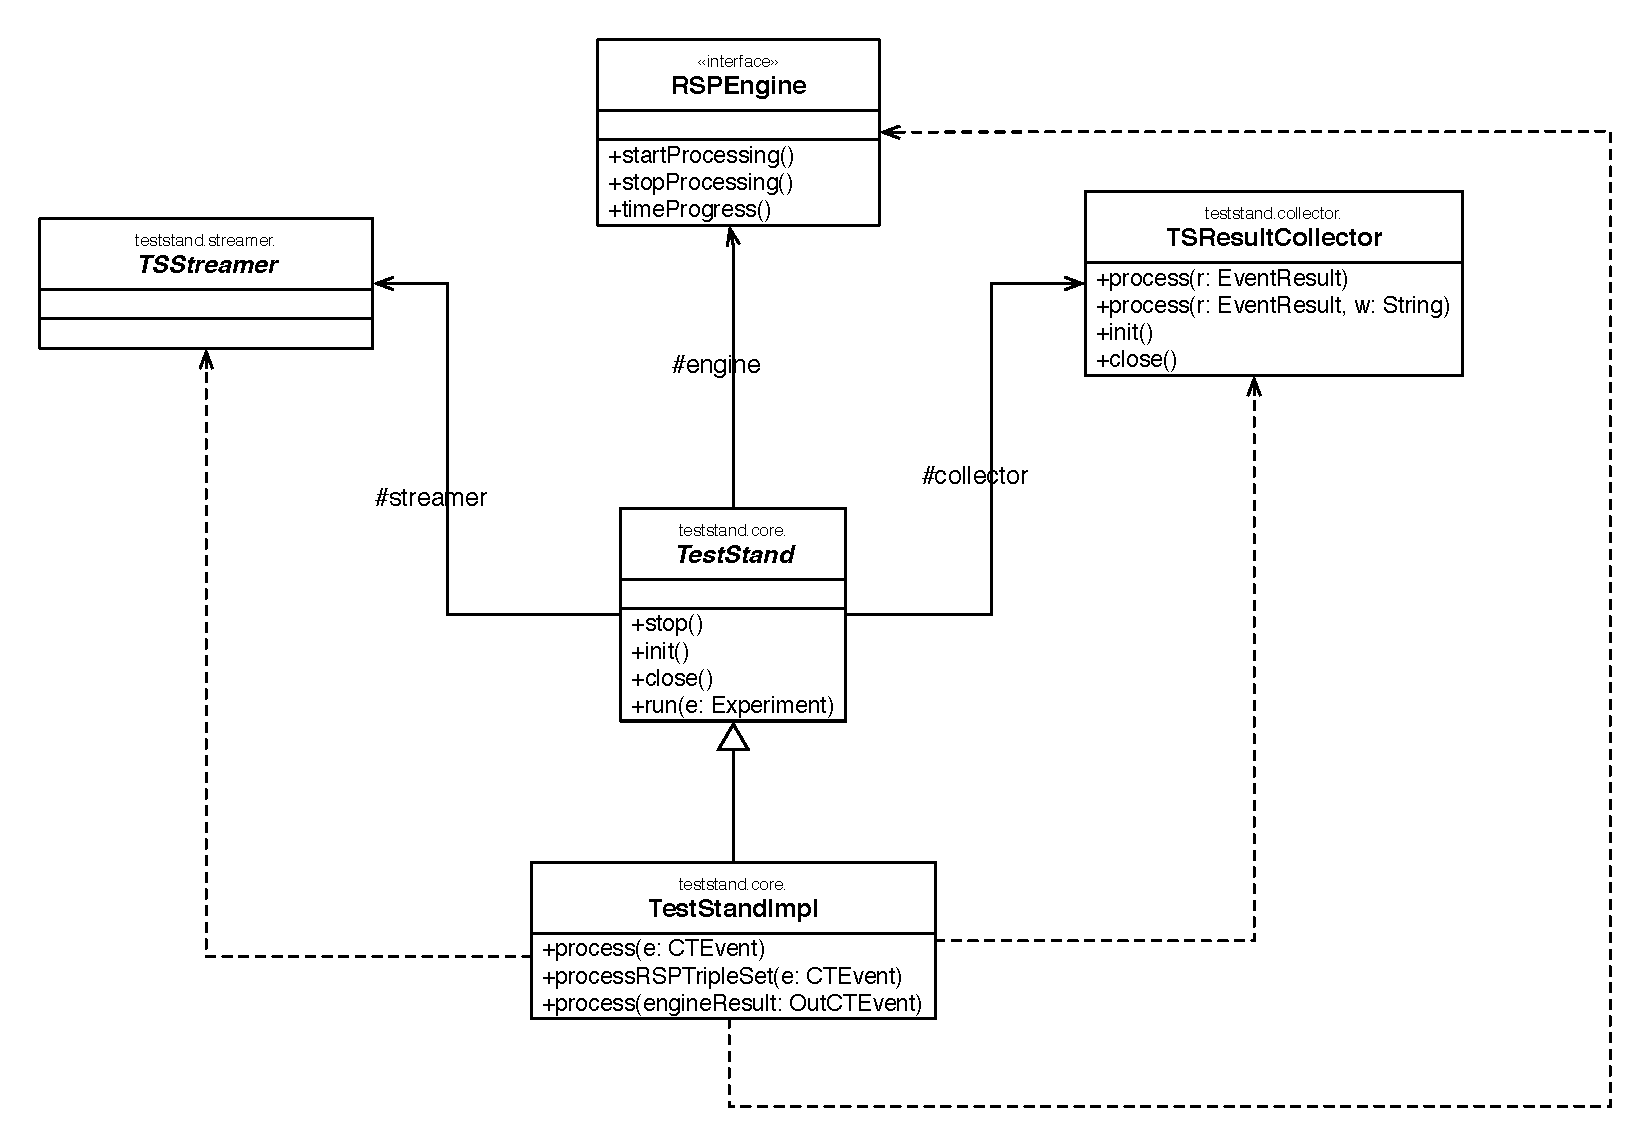
\includegraphics[width=1\linewidth]{images/uml_teststand_modules}
	\caption[\name \textsc{TestStand} and Modules  - UML Schema] {The \textit{TestStand} contains references of the \textit{TSStreamer}, the engine behind the \textit{RSPEngine} interface and the \textit{TSResultCollector}. The \textit{TSStreamer} and current \textit{RSPEngine} are linked to the next element in the pipeline through the \textit{TestStand}. Two arrows, labelled with "next", point to the  \textit{TestStand} indicating that it receives the events from all modules and it orchestrates the communication. The arrow that starts from the \textit{RSPEngine} is coloured in gray to highlight that it can not be seen at this level of detail, because \textit{RSPEngine} is an interface. The \textit{ResultCollector} receives the result to save at the end of each cycle and, when it returns the call, the process ends.} 
  	\label{fig:uml_teststand_modules}
\end{figure}

\pagebreak

\section{Baselines}\label{sec:baselines-impl}

\name Baselines are four elementary implementations of an RSP Engine, which  cover the requirements from [R.13] to [R.16] and implement the pipeline of a DSMS with a reasoner following the proposal presented in Section~\ref{sec:baselines}. 
The RSP Engine pipeline is composed by Esper\footnote{$http://www.espertech.com/esper/$}, a mature commercial DSMS, with the Jena general purpose rule engine\footnote{http://jena.apache.org/documentation/inference/\#rules}, a flexible reasoning engine.  The aim of the choice of Esper and Jena is fulfilling requirement [R.14], baselines Eligibility by coupling two mature solutions for stream processing and reasoning and, thus, obtaining a fair solution in the SR context. Moreover, both Esper and Jena are open source solution, which allow us to release \name as open source too.

\begin{figure}[tbh]
  \centering
	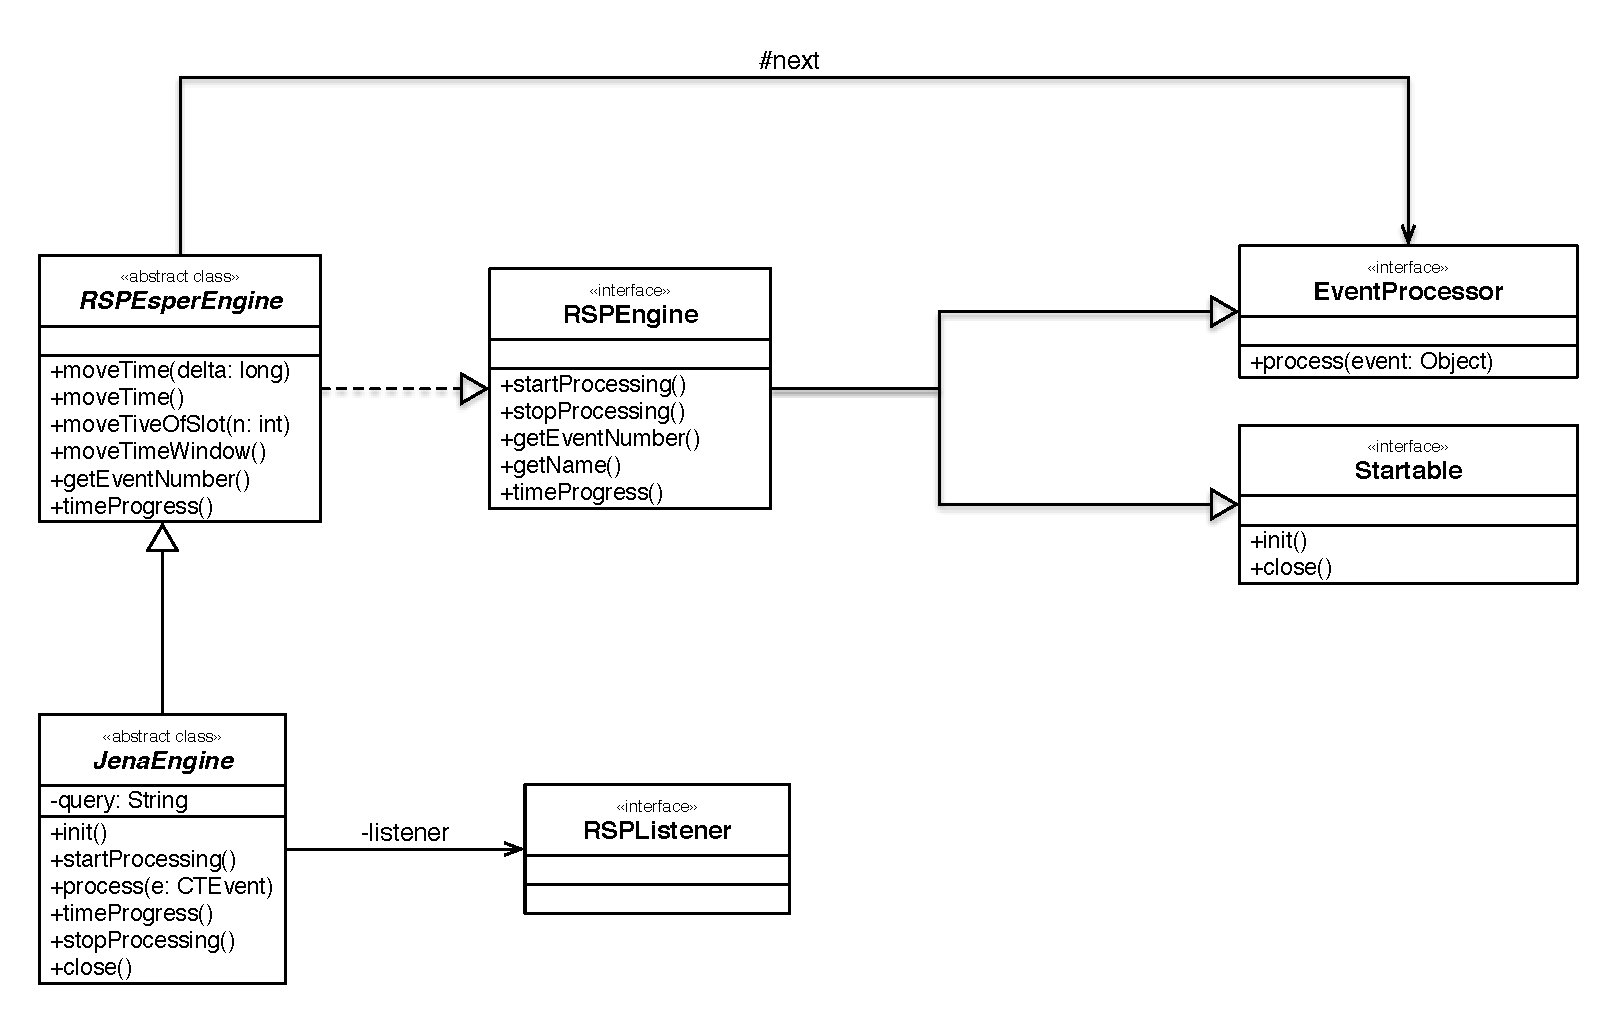
\includegraphics[width=\linewidth]{images/uml_baselines_general}
	\caption[\textit{RSPEngine} Implementation Through Esper and Jena - UML Schema]{The \textit{RSPEngine} interface extends both the \textit{EventProcessor} and the \textit{Startable} one. The \textit{RSPEsperEngine} class implements the interface adding the Esper runtime to handle its internal events. The \textit{JenaEngine} together with the \textit{RSPListener} integrate the Jena reasoning system into the engine.}
  	\label{fig:uml_baselines_general}
\end{figure}

\noindent Figure~\ref{fig:uml_baselines_general} presents how the baselines are implemented. The general structure exploits the \textit{RSPEngine} interface, a proxy for both the \textit{EventProcessor} and the \textit{Startable} interfaces described in Section~\ref{sec:abstractions}. 

\name Baselines integrate Esper as the DSMS, which composes the first half of the RSP Engine pipeline. The \textit{RSPEsperEngine} abstract class implements the \textit{RSPEngine} interface in order to share the Esper runtime definition for all the Baselines.  They exploit the ability of Esper to be temporally controlled by an external agent\footnote{\url{http://esper.sourceforge.net/esper-0.7.5/doc/reference/en/html_single/index.html#api-controlling-time}}. Thus, the internal time flow can be synchronised by sending time-keeping events. In this way, it possible to ensure the complete and soundness of query results, even in case of high traffic load. To enable external time control the \textit{RSPEngine} interface exposes the \textit{moveTime()} method.  The \textit{RSPEsperEngine} implements \textit{moveTime()} encapsulating the logic to send a time-keeping event into Esper: one time-keeping event is sent before injecting the triples within a \textsc{CTEvent} and the next one after all triples in \textsc{CTEvent} were sent. In this way, all the triples in the \textsc{CTEvent} are considered contemporary by the Baselines. 

The RSP Engine is in the middle of the \textsc{Test Stand} pipeline and, thus, it is has to communicate with the following module. The \textit{RSPEsperEngine} has a reference to a general \textit{EventProcessor}, represented in Figure~\ref{fig:uml_baselines_general}  by the arrow labelled as "next", which can be any module which processes \textit{CTEvent}. In the current implementation, the \textsc{Test Stand Supporting Structure}, implemented as the \textit{TestStandImpl} class, follows a \textit{RSP Engine} to intercept the outcoming \textit{OUTCTEvents}.

\begin{figure}[tbh]
  \centering
	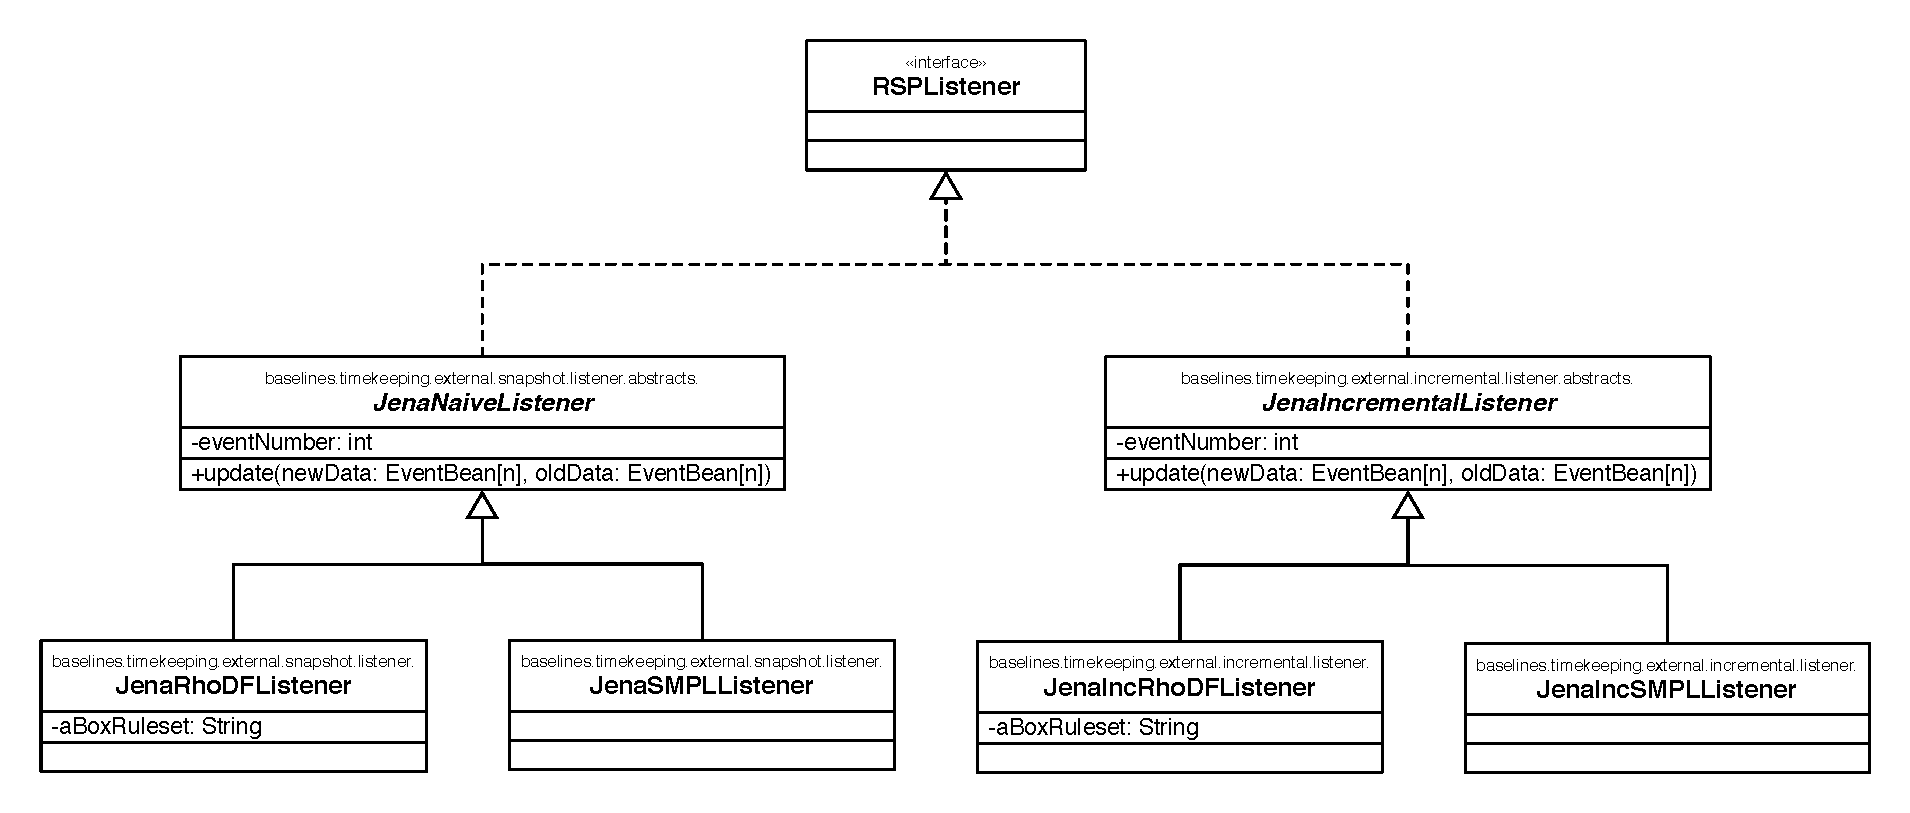
\includegraphics[width=\linewidth]{images/uml_baselines_listener}
	\caption[\textit{RSPListener} Implementations - UML Schema]{The \textit{RSPListener} is actually a proxy for the native Esper \textit{UpdateListener}. We implement the interface following two possible reasoning approaches, Naive and Incremental, respectively into the  \textit{JenaNaiveListener} and the \textit{JenaIncrementalListener}. Further implementations like the \textit{JenaNaiveRhoDFListener} allows to specify to the listeners the entailment regime and the TBox.} 
  	\label{fig:uml_baselines_listener}
\end{figure}

We draw, in Figure~\ref{fig:uml_baselines_general}, the UML schema of the Baseline implementation. The \textit{JenaEngine} abstract class links the DSMS to the reasoner, an thus it requires a further component, the RSPListener, to complete the RSP Engine pipeline and realise the system we describe in Section~\ref{sec:baselines}
 
The reasoner stage is realised as shown in Figure~\ref{fig:uml_baselines_listener}. Different implementations of the listener, which all belong to the \textit{RSPListener} interface, variate the reasoning approaches between Naive or Incremental. The \textit{JenaNaiveListener} or the \textit{JenaIncrementalListener} partially fulfil requirement [R.15] (baseline relevance) in terms of reasoning. None of the two specifies the entailment regime and the TBox, which must be defined with specific implementations like the \textit{JenaRHODFNaiveListener}, as it is visible again in the Figure~\ref{fig:uml_baselines_listener}.

The Baselines relevance, demanded by [R.15], is only partially fulfilled by the alternative reasoning approaches. It comes also from the different implementations of the RDF~Stream model, graph based or triple based. Esper runtime demands to registers the events that it has to handle. Figure~\ref{fig:uml_baselines_events} shows how events are implemented: they belongs to the \textit{JenaEsperEvent} interface, which exposes three methods used by the \textit{RSPListener} to manage the active window independently from the event implementation. The methods \textit{addTo(Graph g)} and \textit{removeFrom(Graph g)} delegate to the event the inserting and deleting operations, in a transparent way for the \textit{RSPListener}; the method \textit{serialise()} unrolls the event into a set of statements, in this way the RSP Engine can output an \textit{OutCTEvent} independently from the RDF Stream implementation: \textit{GraphEvent} or \textit{TripleEvent}

\begin{figure}[t!]
  \centering
	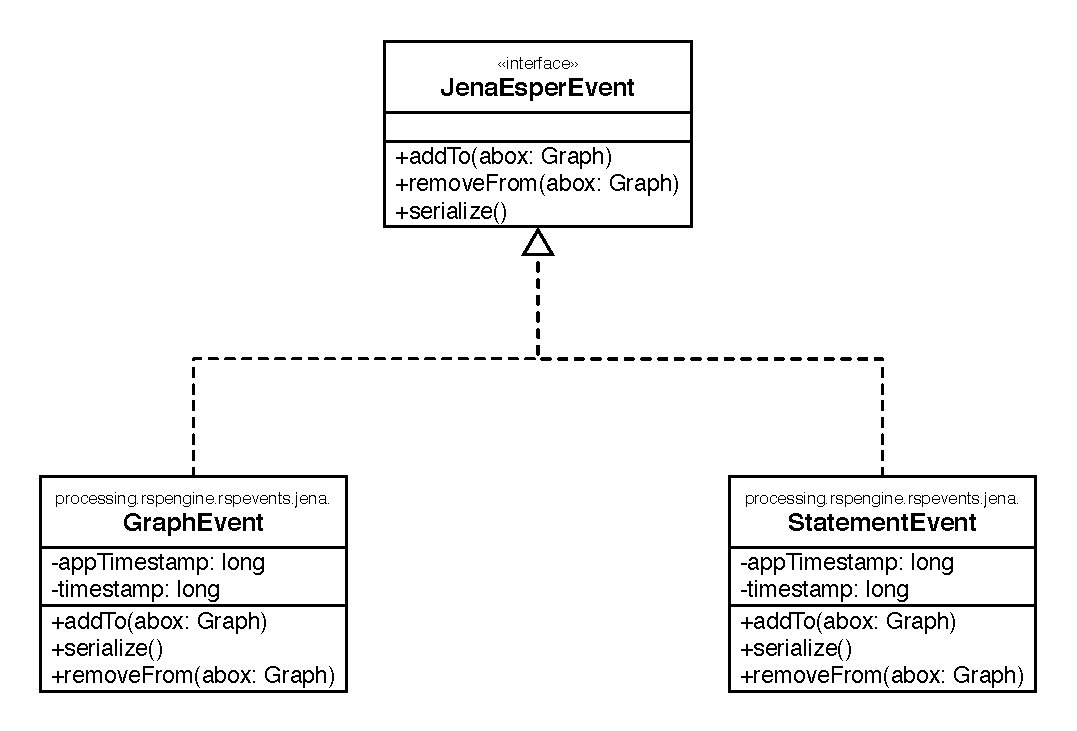
\includegraphics[width=0.8\linewidth]{images/uml_baselines_events}
	\caption[Esper-level Graph based and Triple based - UML Schema]{ All the event registered to Esper belong to the \textit{JenaEsperEvent} interface, which exposes methods to handle the reasoning independently from the RDF Stream implementation:  \textit{GraphEvent} or \textit{TripleEvent}. The triples received by the \textit{RSPEngine} can be pushed into Esper as a complete graph or as a set statements. To handle the active window, independently from the event implementation, the interface exposes the method \textit{addTo(Graph g)} and \textit{removeFrom(Graph g)}, while the \textit{serialise()} methods unroll the event into a set of statements, in order to build an outgoing \textit{OutCTEvent}.}
  	\label{fig:uml_baselines_events}
\end{figure}

When a \textit{CTEvents} comes to the RSP Engine, it will be transformed into the events handled by the DSMS, contained in Figure~\ref{fig:uml_baselines_events}. This translation process influences the latency calculus, because the time spent by the engine to translate events from the RDF~Stream into its internal mechanism may be relevant. Once the processing is complete, the output of the RSP Engine is translated again into an \textit{OutCTEvent} and passed to the next \textit{EventProcessor}, again spending time that influences the latency. 

This assumption is inspired by the related work \cite{bizarro:DSP:2007:1143}, which endorses the idea of black box testing provided by \namens. \cite{bizarro:DSP:2007:1143} states that every buffering or translation process, which is applied by the engine in use, must be considered part of its internal mechanism and, thus, part of the performance measurement.

The current Baseline implementations divide the different architectural elements and delegate to each element a specific task to share the majority of the code and thus fulfilling [R.16], which demands baseline Simplicity.

%\begin{figure}[tbh]
%  \centering
%	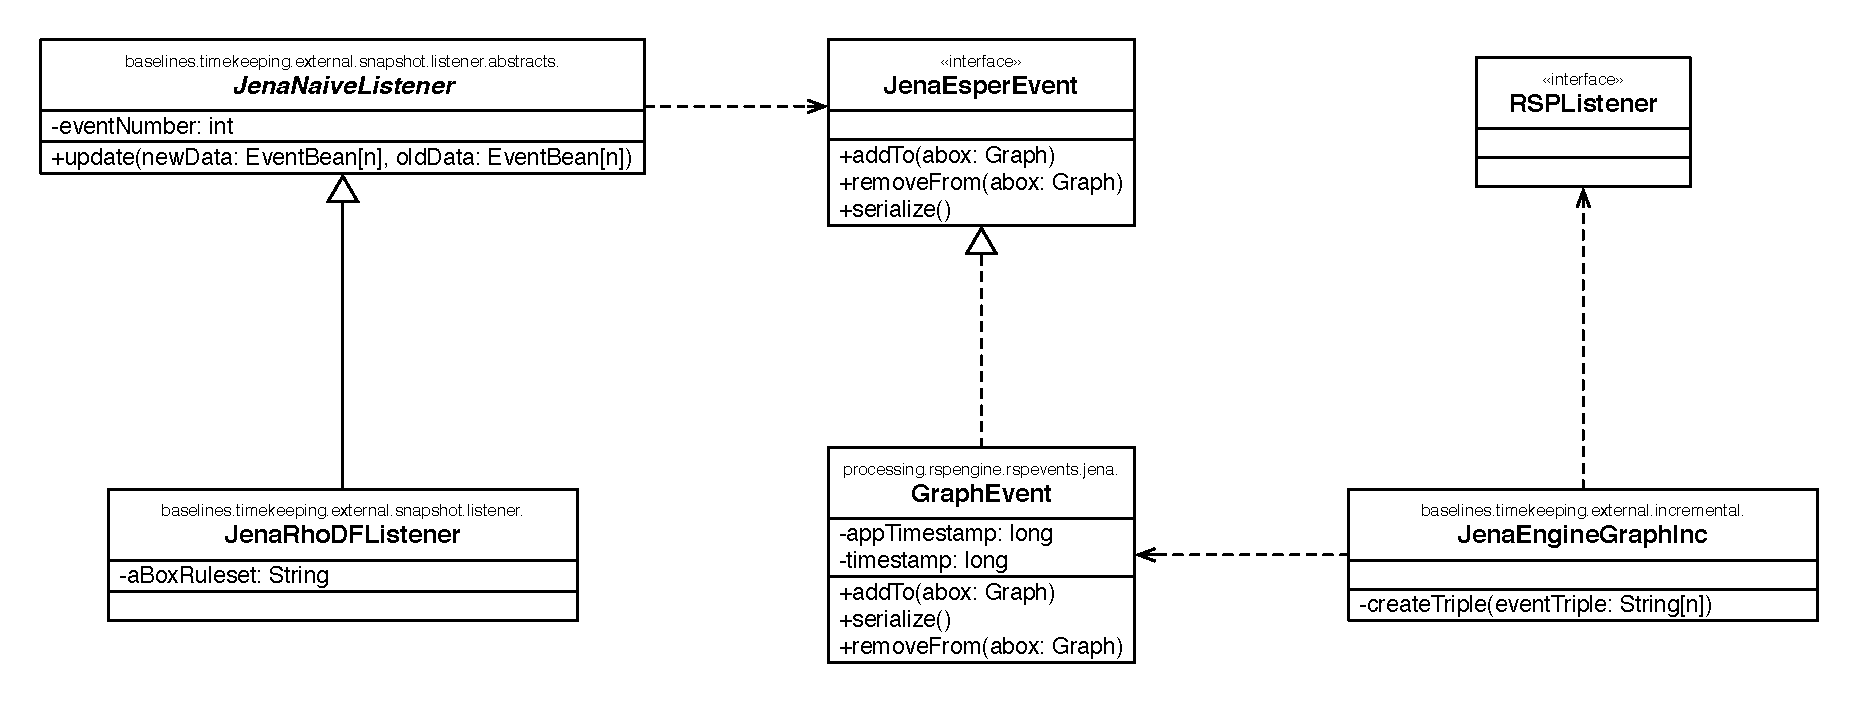
\includegraphics[width=\linewidth]{images/uml_baselines_rel_listener_event}
%	\caption[The Relation between \textit{RSPListener} and \textit{JenaEsperEvent} - UML Schema]{The listener and the event implementation are fully decoupled but logically related. In picture is detailed this relation for different implementation of the \textit{RSPListener}}
%  	\label{fig:uml_baselines_rel_listener_event}
%\end{figure}
%
%\textit{\textit{JenaNaiveListener} and the  \textit{JenaIncrementalListener} handle the events which come form the DSMS through the \textit{JenaEsperEvent} interface, Figure~\ref{fig:uml_baselines_rel_listener_event} report  the structure for the case of Graph-based event representation (see Section~\ref{sec:baselines} for event details). }

\pagebreak

\section{Analyser}\label{sec:analyser-impl}

\begin{figure}[tbh]
  \centering
	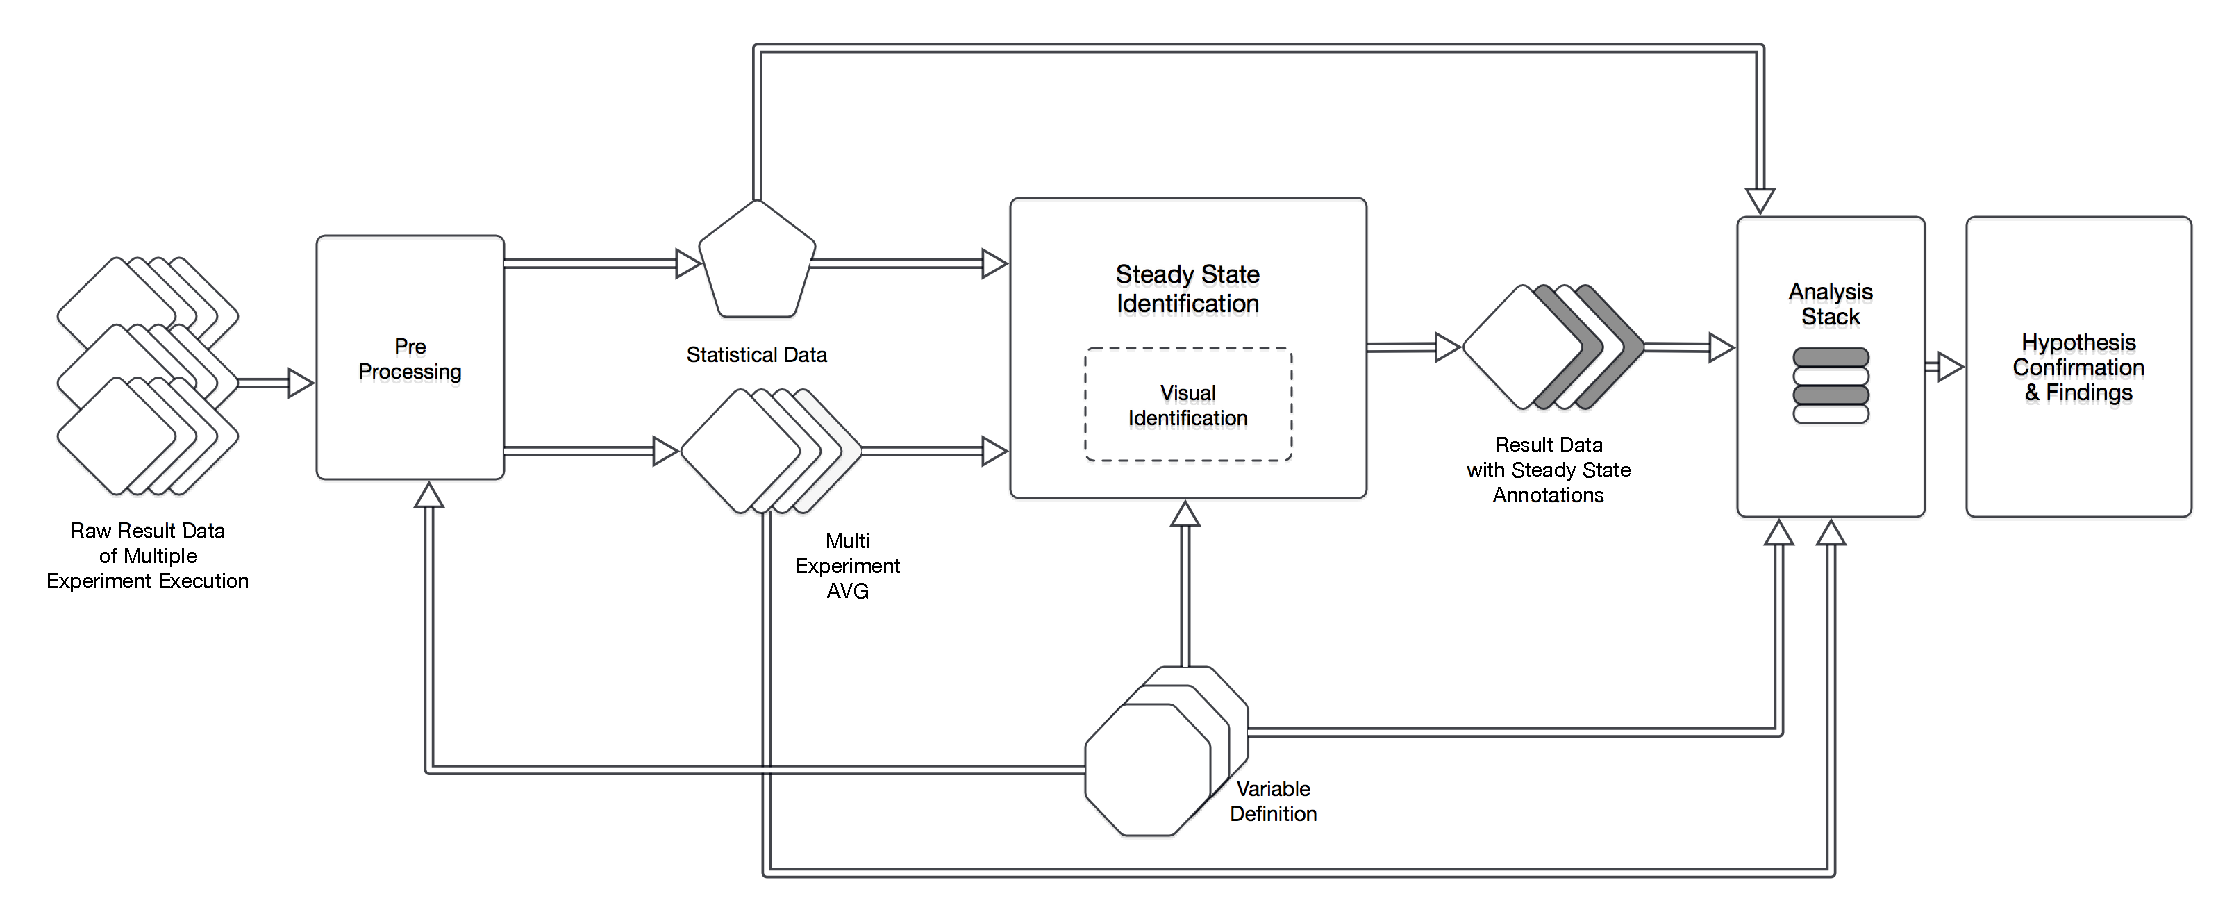
\includegraphics[width=\linewidth]{images/analyser-block-schema-impl}
	\caption[\textsc{Analyser} Block Schema: Implementation Detail Level]{The \textsc{Analyser} block schema in figure extends the one in Figure~\ref{fig:analyser-block-schema}, with several implementation details. In particular, a new initial block, named \textit{Pre-Processing}, operates before the other ones on the experiment raw data: it averages among multiple executions of the same experiment, to obtain a single reliable dataset; it calculates statistical relevant values (maximum, minimum, median etc) for each experiment w.r.t the involved variables that it receives as input. The \textit{Pre-Processing} outputs are consumed by both the \textit{Steady State Identification} block and the \textit{Analysis} block.}
  	\label{fig:analyser-block-schema-impl}
\end{figure}

\noindent In this section, we introduce which analysis tools sustain each level in the investigation stack described in Section~\ref{sec:analyser} and how they are realized in the current implementation of \namens. 

The relation between the hypothesis and the tools that sustain the analysis is deep and, thus, it is hard to generalise the investigation toolset. The Hypothesis depend on the the research question, while the tools are related to the nature of the data and to the experiment. However, there are several genera characteristics, which are meaningful independently from both the hypothesis and experiment. Thus, we can develop a basic toolset which sustains the entire investigation stack presented in Section~\ref{sec:analyser}.

Figure~\ref{fig:analyser-block-schema-impl} shows the different phases of data processing. It refers to the original block schema presented in Chapter~\ref{chap:heaven}, but Figure~\ref{fig:analyser-block-schema-impl} provides further implementation details.\\ 

The Figure~\ref{fig:analyser-block-schema-impl} shows the \textsc{Analyser} receives two inputs:
\begin{itemize}
\item the raw data form the experiments,
\item the variables to build the analysis.
\end{itemize}

In the original block schema, (see Figure~\ref{fig:analyser-block-schema}) both inputs directly enter the \textit{Steady State Identification} block (SSI) and the \textit{Analysis} block (AB). In Figure~\ref{fig:analyser-block-schema-impl} instead, the first block in the process is the \textit{Pre-Processing} block. Empirical analysis can not rely on a single execution of an experiment, because even if the \textit{Test Stand} is designed to be system independent, we do not have the complete control of the active processes within the execution environment. Strange behaviours may happen while an experiment is running. In order to reduce, and possibly eliminate, the outliers, multiple runs of the same experiment must be mediated obtaining the average measures. The \textit{Pre-Processing} block ensures data reliability extrapolating a unique dataset from multiple executions. Moreover, time series describes how a dynamic system evolves over time, so it is meaningful to attempt hypothesis verification through statistical values, which always consider the the Steady State to allow the generalisation of the insights. The \textit{Pre-Processing} block calculates most common statistical metrics as average, standard deviation and maximum or minimum for a certain variable.

%Indeed, both the Steady State Identification Block and Analysis Block require an automatic procedure, named pre-processing in Figure~\ref{fig:analyser-block-schema-impl}, which averages the data of multiple executions of the same experiment and calculate the statistically relevant data. 

Once we have reliable data, the \textit{Steady State Identification} block and the \textit{Analysis} block cans start the analysis process on the input variables and the \textit{Pre-Processing} outputs. 

Finally, researches can read the analysis point out insight and theoretical results as the last block in the process describes.

%We include in Chapter~\ref{chap:evaluation} concrete analysis examples, by testing the Baselines. The aim of Chapter~\ref{chap:evaluation} is to demonstrate the value of \namens, but also we want to provide some guidelines for further evaluations.

The following sections contain further details about the \textit{Steady State Identification} block implementation, Section~\ref{sec:analyser-impl-ss-block}, and about the \textit{Analyser} block with the investigation stack, Section~\ref{sec:analyser-impl-analysis-block}.

\subsection{Steady State Identification Block}\label{sec:analyser-impl-ss-block}

The Steady State Identification block aims of determining if a a certain variable has reached the Steady State condition (see Section~\ref{sec:analyser-analysis-block}). Automatic procedures to identify the State State condition exist, but they require dedicated studies, which will be faced as future works. Currently, the SSI block is not automated. It exploits data visualisation techniques, to identify if and when a variable reaches the Steady State condition. We plot each variable trend in the time domain over all the experiment execution. Then, we manually exclude the initial warm-up phase from the data evaluation.

We know that the graphical method is limited, because it must be applied for each system variable, and human criteria cannot be reliable in this kind of analysis as automatic procedures, which exploit tested algorithms. Moreover, different variables may reach the equilibrium at different times, so it is researcher responsibility to properly identify the different conditions for each variable involved. Thus, we include this further development as future work.

\subsection{Analysis Block}\label{sec:analyser-impl-analysis-block}

\noindent The \textsc{Analyser} block includes five analysis levels, (see Section~\ref{sec:analyser} with increasing degrees of detail, and where the comparative research approach is declined either via visual analysis or statistical investigation. The graphical analysis method is more qualitative then the statistical one, but reading the information presented in graphical way can be preferred in those cases where numerical data are not so meaningful. On the other hand, the statistical investigation method demands more complex instruments to obtain the data, but they allow to answer also more elaborate questions. In the following, we present the current implementation of all the analysis levels.

\subsubsection{Level 0 - Dashboards}\label{sec:impl-level0}

\begin{figure}[h!tbp]
  \centering
	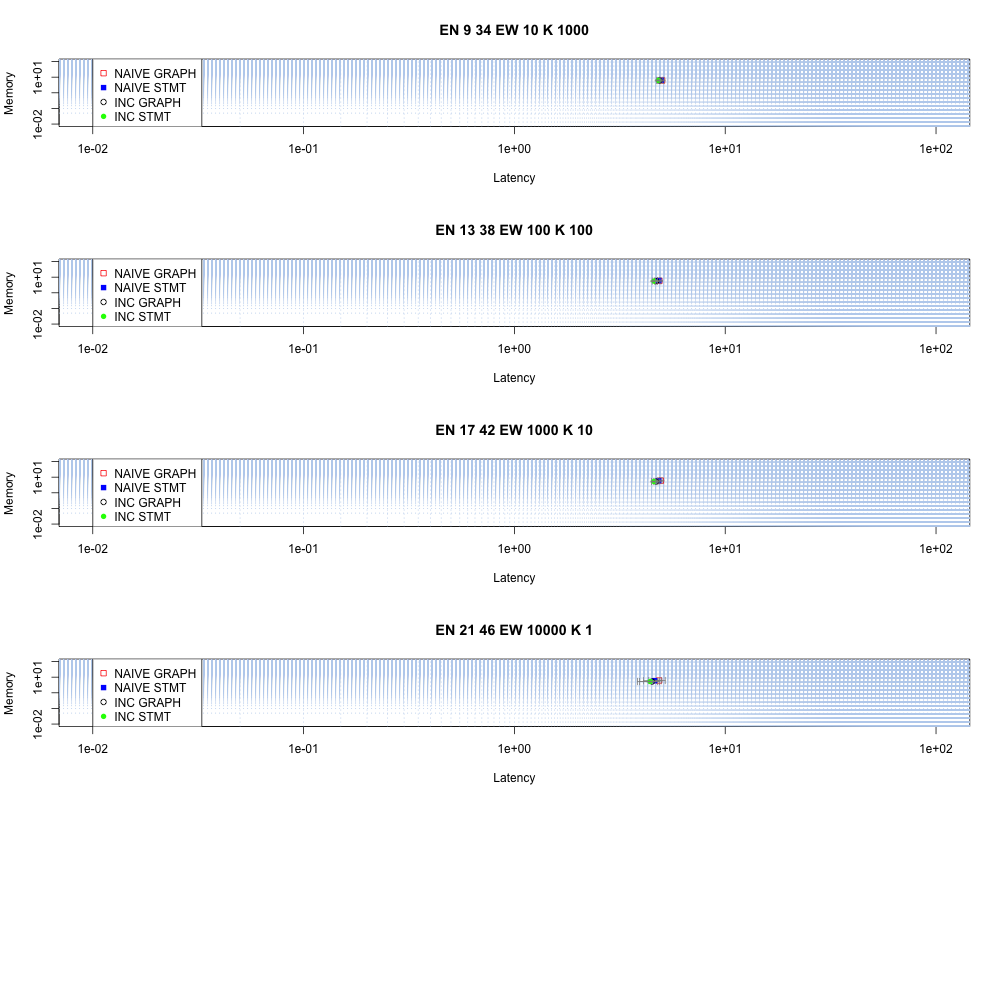
\includegraphics[width=0.6\linewidth]{images/dashboard-example}
	\caption[\textsc{Analyser} Investigation Stack - Level 0 -  Dashboard Representation Examples]{\textsc{Analyser} Investigation Stack - Level 0 -  Dashboard Representation Examples.}
  	\label{fig:dashboard-example}
\end{figure}

\noindent Figure~\ref{fig:dashboard-example} contains an example of the possible Dashboard representations. We implement the dashboard to represent data on a bi-dimensional Cartesian space where memory and latency are the axis of the graph. This kind of representation allows to define solution dominance, w.r.t the involved variable, through inter-experiment comparisons. Thus, we can easily state which RSP Engine, if any, is better then another.

\subsubsection{Level 1 - Statistical Values Comparison}\label{sec:impl-level1}

Tables~\ref{tab:comp-tables} (a) and (b) show two examples of statistical investigation. Table~\ref{tab:comp-tables}.a contains the qualitative comparison of two solution over a given variable, while Table~\ref{tab:comp-tables}.b offers a deeper detail level, the quantitative comparison, showing how much a solution is better than an other. How to choose the proper level depends on the needs of the research.

\begin{table}[htb]
\scriptsize
	\centering
	\subtable[Symbolic Comparison of variables A vs B on Experiment 1]{%
		\begin{tabular}{c | cccc} % creating eight columns
	  	\hline
		A vs B & \multicolumn{4}{c}{Experiment 1 Condition A}  \\
		 Comparison  & &&&\\
		\hline
		   	        & $\simeq$\\
		 Experiment 1 & A     & 	$\simeq$  & A & B\\
		 Condition  & A     & 	$\simeq$  & $\simeq$ & B\\
		 B          & A     & 	$\simeq$  & B & A\\
		\hline % inserts single-line
	 \end{tabular}
	}\qquad\qquad
	\subtable[Symbolic Comparison of variables A vs B on Experiment 1]{%
		\begin{tabular}{c | cccc} % creating eight columns
	  	\hline
		A vs B & \multicolumn{4}{c}{Experiment 1 Condition A}  \\
		 Comparison  & &&&\\
		\hline
		   	        & $\simeq$\\
		 Experiment 1 & 10\%     & 	$\simeq$  & 42\% & 33\%\\
		 Condition  & 23\%     & 	$\simeq$  & $\simeq$ & 12\%\\
		 B          & 20\%    & 	$\simeq$  & 22\% & 22\%\\
		\hline % inserts single-line
	 \end{tabular}
	}
	\caption[\textsc{Analyser} Investigation Stack - Level 1 - Qualitative and Quantitative Comparison Examples]{\textsc{Analyser} Investigation Stack - Level 1 - Example of qualitative-comparison over two variables  (a)  and  quantitative-comparison over a common variable (b).}
	\label{tab:comp-tables}
\end{table}

Table layout is a key-point for Level 1 representations. Table axes represent the variation of two different experiment properties A and B. Different experiments influence the behaviour of an RSP Engine in different ways, and Level 1 allows to point out this differences with  \textit{Inter-Experiment} comparisons. Thus, we can move on the horizontal axis of Table~\ref{tab:comp-tables}.a, which means variate the Condition A, to appreciate those differences. 

Actually this kind of analysis is possible thanks to a report, which contains all the meaningful statistical values for the experiments. The report can be further manipulated to obtain the table visualisation.

\subsubsection{Level 2 - Patter Identification}\label{sec:impl-level2}

%\begin{figure}[tbh]
%  \centering
%   \subfigure[Pattern Recognition Example: Memory in Time Domain]{
%  	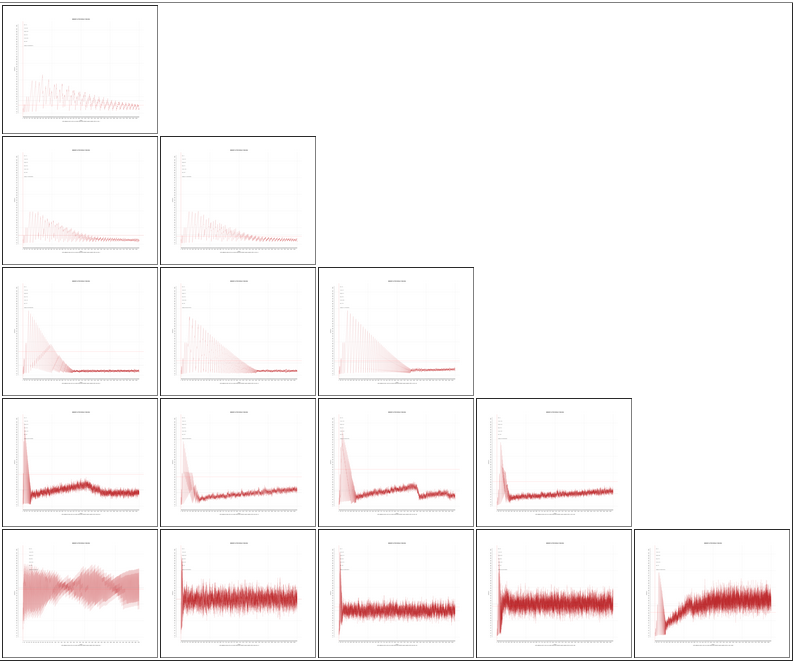
\includegraphics[width=0.45\linewidth]{images/pattern-example-memory}
%  }
%  \subfigure[Pattern Recognition Example: Memory Distribution]{
%  	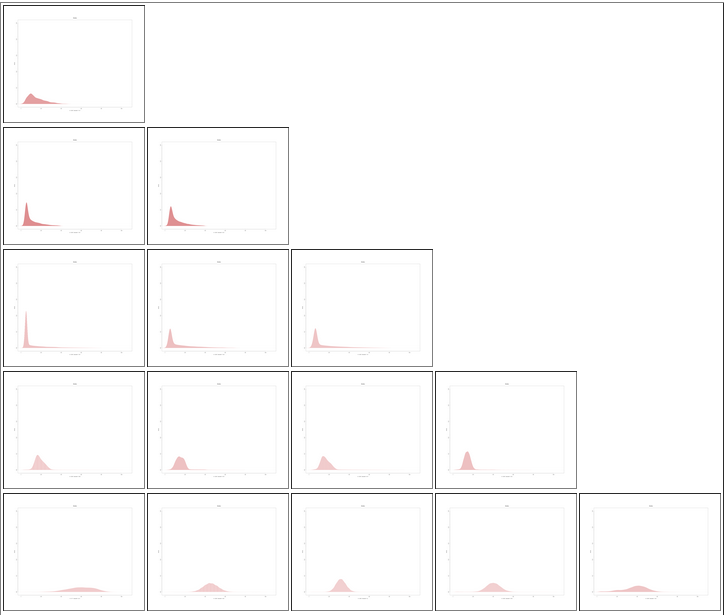
\includegraphics[width=0.45\linewidth]{images/pattern-example-density}
%  	
%  }
%   %\subfigure[Pattern Appear On the Wall..]{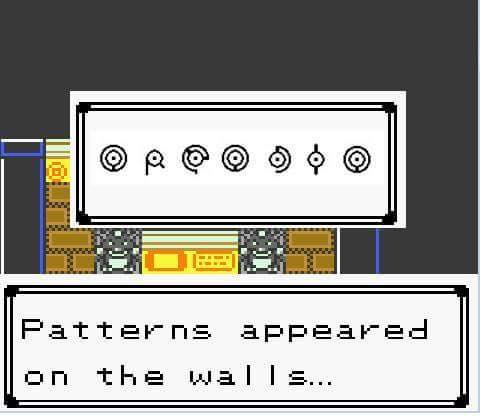
\includegraphics[width=0.45\linewidth]{images/pokepattern}}
%	\caption[\textsc{Analyser} Investigation Stack - Level 2 - Pattern Recognition Examples]{Two examples of pattern recognition. Level 2 exploits  easy-to-read layouts which highlights the experiment difference to enable \textit{Inter Experiment} comparisons} 
%  	\label{fig:pattern-examples}
%\end{figure}

\begin{table}[htbp]
	\centering
	\scriptsize
	\subtable[Pattern Recognition Example: Memory Time Domain]{%
		\begin{tabular}{l | ccccc} % creating eight columns
	  	\hline
		Triple  & \multicolumn{5}{c}{Slots}  \\
		in & \multicolumn{5}{c}{Number}  \\
		Window  & 1 & 10 & 100 & 1000&10000\\
		\hline
		1	   &\begin{minipage}{.1\textwidth}
     			 	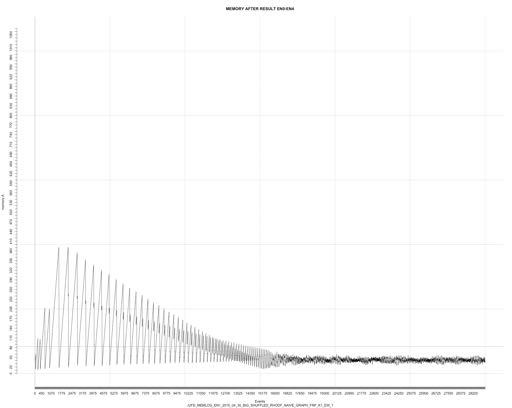
\includegraphics[width=\linewidth]{images/mema-graph/N1}
    				 \end{minipage}\\			
		10	   & \begin{minipage}{.1\textwidth}
     			 	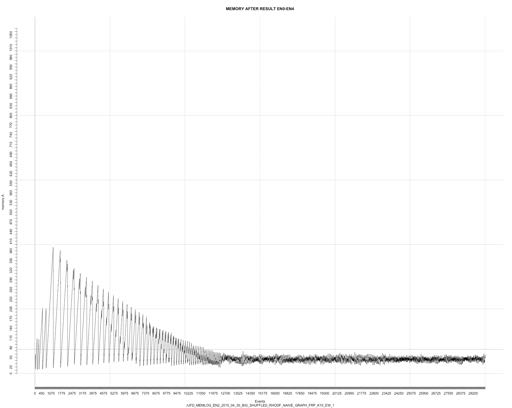
\includegraphics[width=\linewidth]{images/mema-graph/N2}
    				\end{minipage}
    			   & \begin{minipage}{.1\textwidth}
     			 	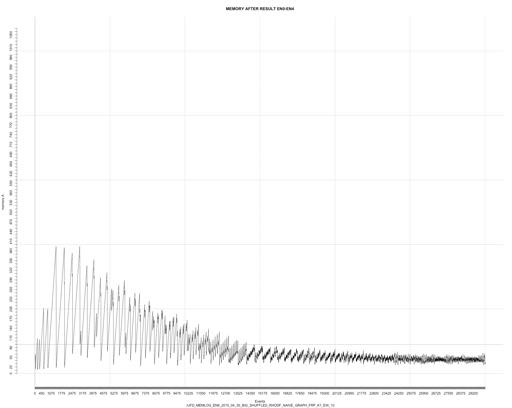
\includegraphics[width=\linewidth]{images/mema-graph/N6}
    				 \end{minipage}\\		
		100	   & \begin{minipage}{.1\textwidth}
     			 	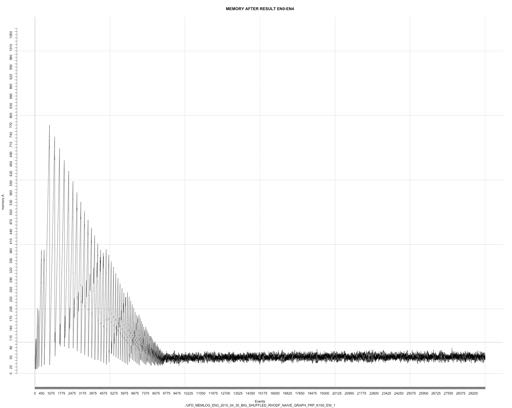
\includegraphics[width=\linewidth]{images/mema-graph/N3}
    				 \end{minipage}
    			   & \begin{minipage}{.1\textwidth}
     			 	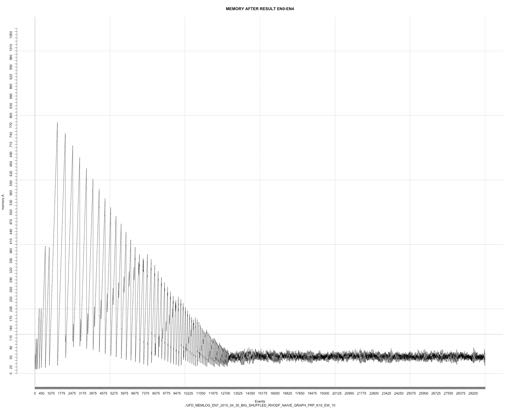
\includegraphics[width=\linewidth]{images/mema-graph/N7}
    				 \end{minipage}
    			   &	 \begin{minipage}{.1\textwidth}
     			 	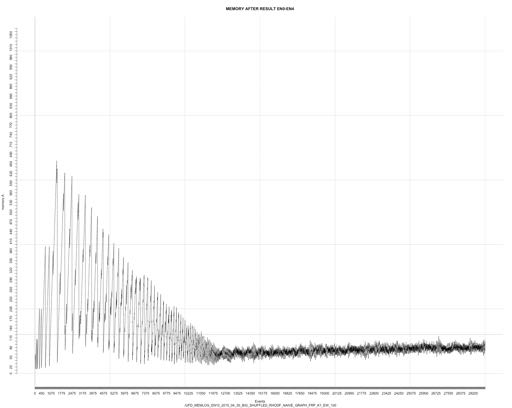
\includegraphics[width=\linewidth]{images/mema-graph/N10}
    				 \end{minipage}\\	
		1000   &	 \begin{minipage}{.1\textwidth}
     			 	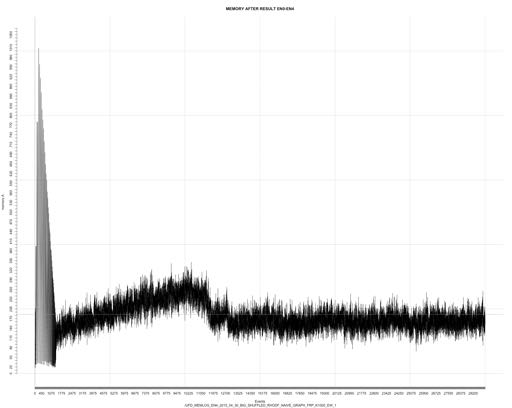
\includegraphics[width=\linewidth]{images/mema-graph/N4}
    				 \end{minipage}
    			   &	 \begin{minipage}{.1\textwidth}
     			 	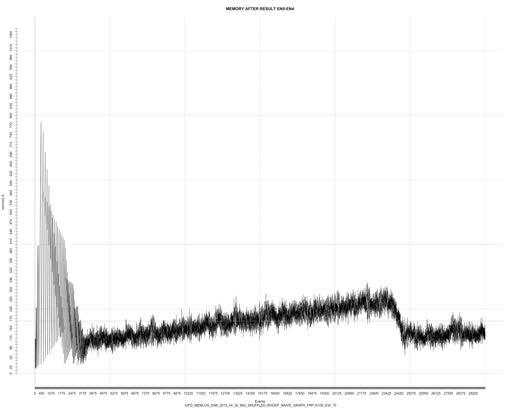
\includegraphics[width=\linewidth]{images/mema-graph/N8}
    				 \end{minipage}
    			   &	 \begin{minipage}{.1\textwidth}
     			 	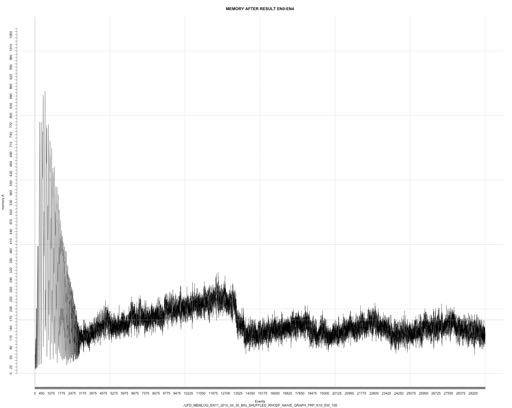
\includegraphics[width=\linewidth]{images/mema-graph/N11}
    				 \end{minipage}
    			   &	 \begin{minipage}{.1\textwidth}
     			 	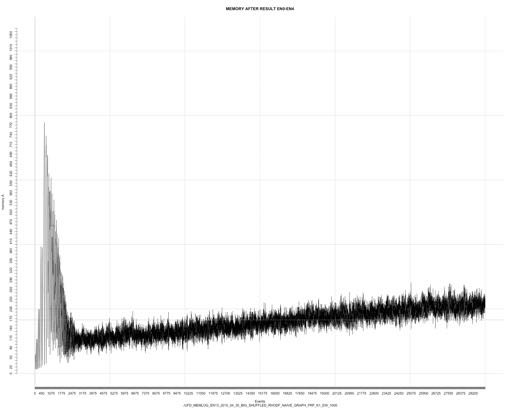
\includegraphics[width=\linewidth]{images/mema-graph/N13}
    				 \end{minipage}\\
		10000  &	 \begin{minipage}{.1\textwidth}
     			 	
\includegraphics[width=\linewidth]{images/mema-graph/N5}
    				 \end{minipage}
    			   &	 \begin{minipage}{.1\textwidth}
     			 	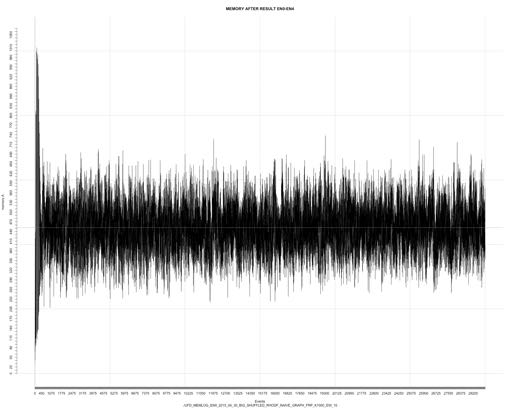
\includegraphics[width=\linewidth]{images/mema-graph/N9}
    				 \end{minipage}
    			   &	 \begin{minipage}{.1\textwidth}
     			 	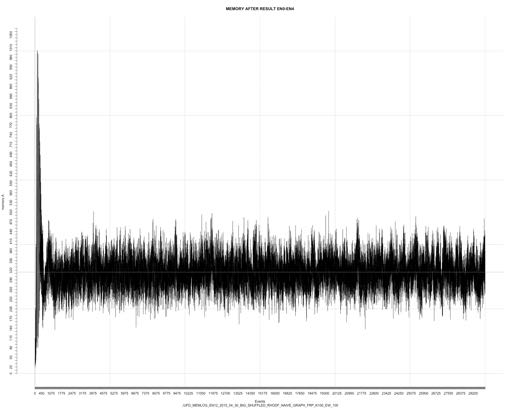
\includegraphics[width=\linewidth]{images/mema-graph/N12}
    				 \end{minipage}
    			   &	 \begin{minipage}{.1\textwidth}
     			 	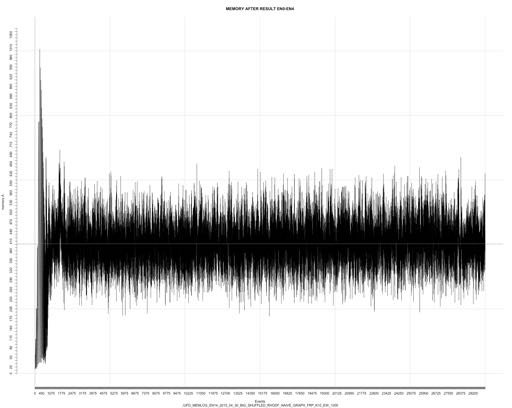
\includegraphics[width=\linewidth]{images/mema-graph/N14}
    				 \end{minipage}
    			   &	 \begin{minipage}{.1\textwidth}
     			 	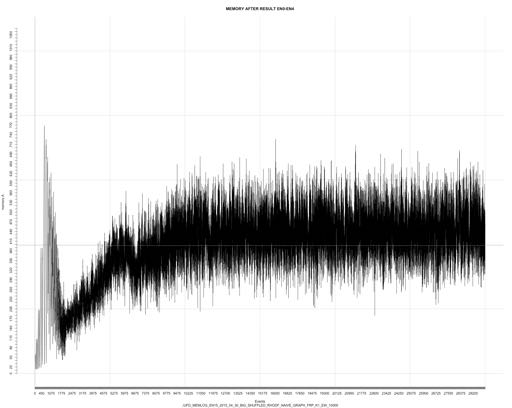
\includegraphics[width=\linewidth]{images/mema-graph/N15}
    				 \end{minipage}\\
		\hline % inserts single-line
	 \end{tabular}
	}
	\subtable[Pattern Recognition Example: Memory Distribution]{%
		\begin{tabular}{l | ccccc} % creating eight columns
	  	\hline
		Triple  & \multicolumn{5}{c}{Slots}  \\
		in & \multicolumn{5}{c}{Number}  \\
		Window  & 1 & 10 & 100 & 1000&10000\\
		\hline
		1	   &\begin{minipage}{.1\textwidth}
     			 	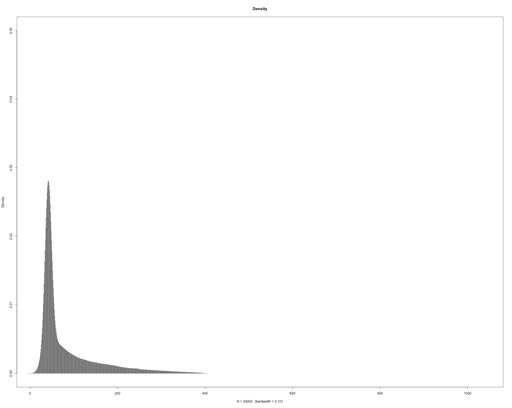
\includegraphics[width=\linewidth]{images/mema-dens-graph/N1}
    				 \end{minipage}\\			
		10	   & \begin{minipage}{.1\textwidth}
     			 	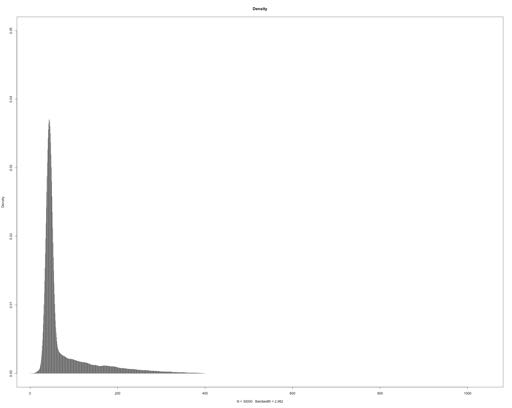
\includegraphics[width=\linewidth]{images/mema-dens-graph/N2}
    				\end{minipage}
    			   & \begin{minipage}{.1\textwidth}
     			 	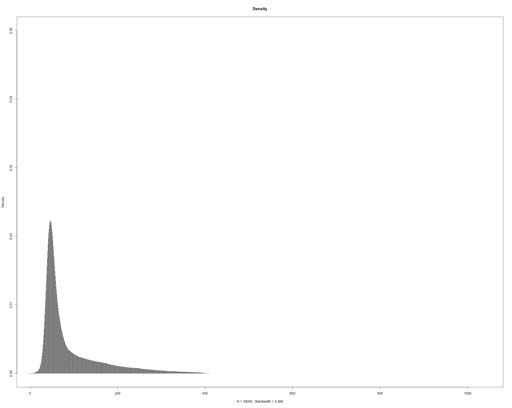
\includegraphics[width=\linewidth]{images/mema-dens-graph/N6}
    				 \end{minipage}\\		
		100	   & \begin{minipage}{.1\textwidth}
     			 	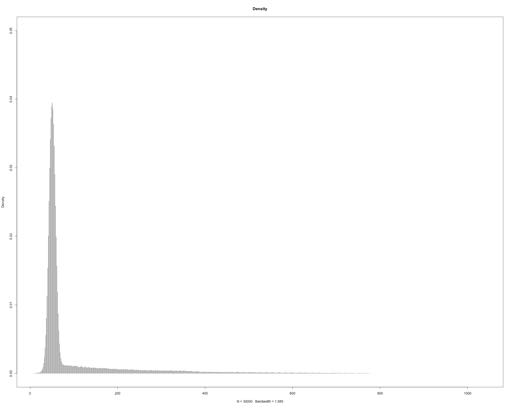
\includegraphics[width=\linewidth]{images/mema-dens-graph/N3}
    				 \end{minipage}
    			   & \begin{minipage}{.1\textwidth}
     			 	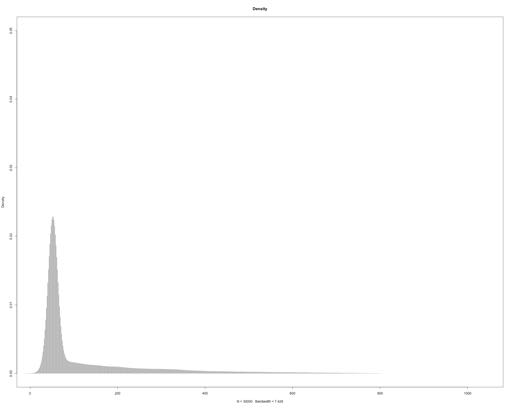
\includegraphics[width=\linewidth]{images/mema-dens-graph/N7}
    				 \end{minipage}
    			   &	 \begin{minipage}{.1\textwidth}
     			 	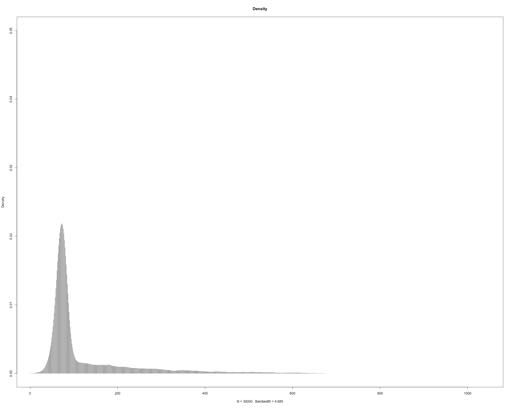
\includegraphics[width=\linewidth]{images/mema-dens-graph/N10}
    				 \end{minipage}\\	
		1000   &	 \begin{minipage}{.1\textwidth}
     			 	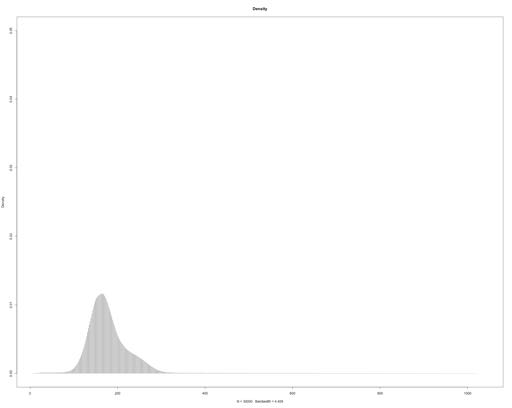
\includegraphics[width=\linewidth]{images/mema-dens-graph/N4}
    				 \end{minipage}
    			   &	 \begin{minipage}{.1\textwidth}
     			 	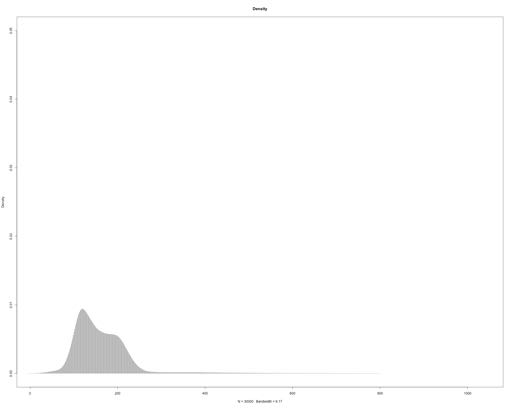
\includegraphics[width=\linewidth]{images/mema-dens-graph/N8}
    				 \end{minipage}
    			   &	 \begin{minipage}{.1\textwidth}
     			 	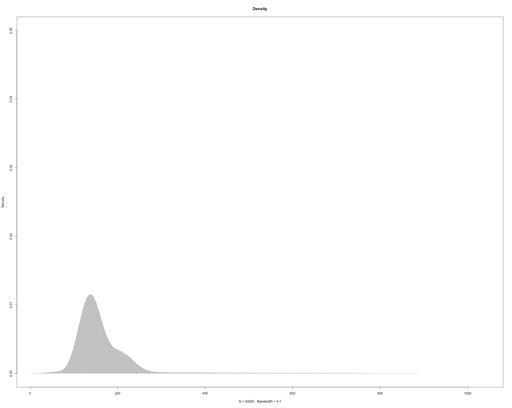
\includegraphics[width=\linewidth]{images/mema-dens-graph/N11}
    				 \end{minipage}
    			   &	 \begin{minipage}{.1\textwidth}
     			 	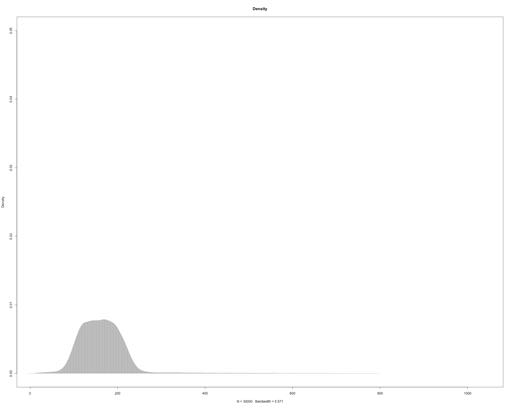
\includegraphics[width=\linewidth]{images/mema-dens-graph/N13}
    				 \end{minipage}\\
		10000  &	 \begin{minipage}{.1\textwidth}
     			 	
\includegraphics[width=\linewidth]{images/mema-dens-graph/N5}
    				 \end{minipage}
    			   &	 \begin{minipage}{.1\textwidth}
     			 	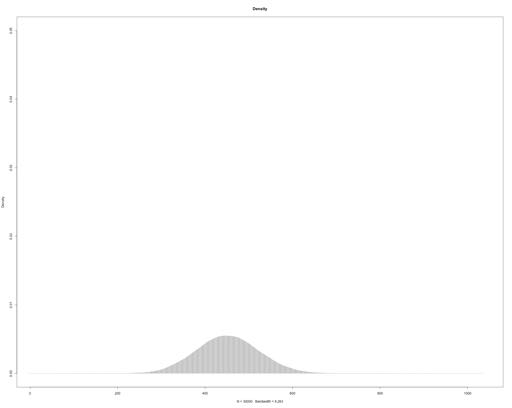
\includegraphics[width=\linewidth]{images/mema-dens-graph/N9}
    				 \end{minipage}
    			   &	 \begin{minipage}{.1\textwidth}
     			 	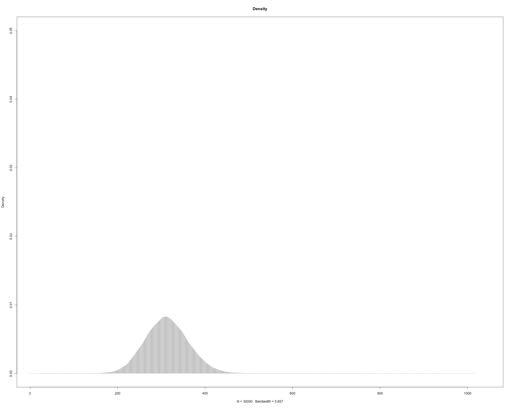
\includegraphics[width=\linewidth]{images/mema-dens-graph/N12}
    				 \end{minipage}
    			   &	 \begin{minipage}{.1\textwidth}
     			 	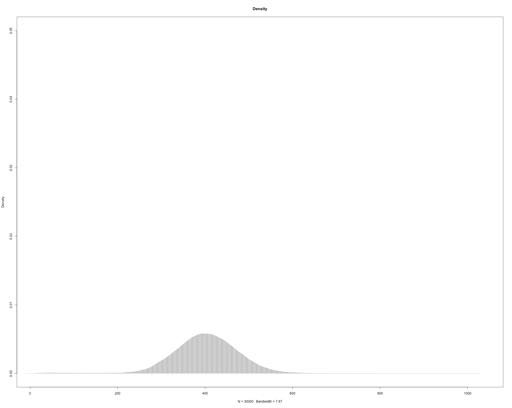
\includegraphics[width=\linewidth]{images/mema-dens-graph/N14}
    				 \end{minipage}
    			   &	 \begin{minipage}{.1\textwidth}
     			 	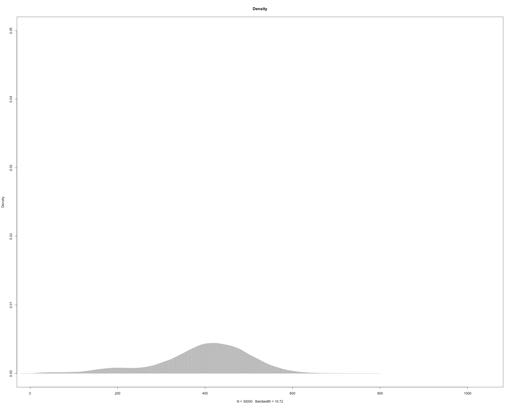
\includegraphics[width=\linewidth]{images/mema-dens-graph/N15}
    				 \end{minipage}\\
		\hline % inserts single-line
	 \end{tabular}
	}
	\caption[\textsc{Analyser} Investigation Stack - Level 2 - Pattern Recognition Examples]{Two examples of pattern recognition. Level 2 exploits  easy-to-read layouts which highlights the experiment difference to enable \textit{Inter Experiment} comparisons} 
	\label{tab:pattern-examples}	
\end{table}

\noindent Level 2 exploits the same experiment layout of Level 1 to compare many graphical representation of the experiment variable. Two examples of memory analysis at Level 2 are reported in Tables~\ref{tab:pattern-examples} (a) and (b). Table~\ref{tab:pattern-examples}.a show the memory behaviour in time domain. It allows to answer questions like "How does the system change the memory behaviour modifying the input dimension?". Table~\ref{tab:pattern-examples}.b reports the memory distribution  values upon several intervals. It allows to understand how memory distribution is influenced by changing the variable on the table axes or diagonals.

Level 3 aims at pattern identification for a given variable. It is an example of \textit{Inter-Experiment} comparison which enables a new kind of global analysis, because it requires to state observation upon the entire set of experiment.

\subsubsection{Level 3 - Visual Comparison}\label{sec:impl-level3}

\noindent Finally, Level 3 focuses on single graphical visualisation. Figure~\ref{fig:visual-comp} contains two examples of the possible analysis. Figure~\ref{fig:visual-comp}.a shows a case of \textit{Inter Experiment} comparison, highlighting the relation between the same variable over multiple experiments; Figure~\ref{fig:visual-comp}.b provides an example of \textit{Intra Experiment} comparison, highlighting the relation between memory and latency within the same experiment.

\begin{figure}[tbh]
  \centering
  \subfigure[Multi-Experiment Comparison]{
  			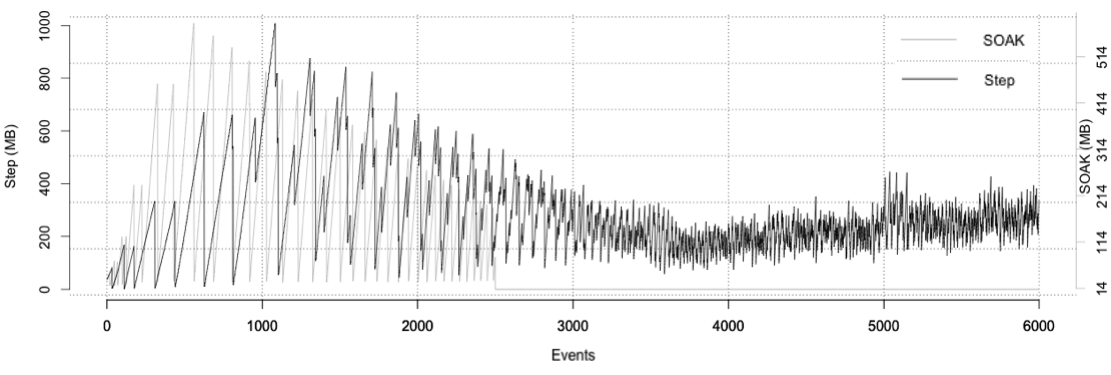
\includegraphics[width=0.70\linewidth]{images/comp-inter}
  			}
  \subfigure[Multi-Variables Comparison]{
  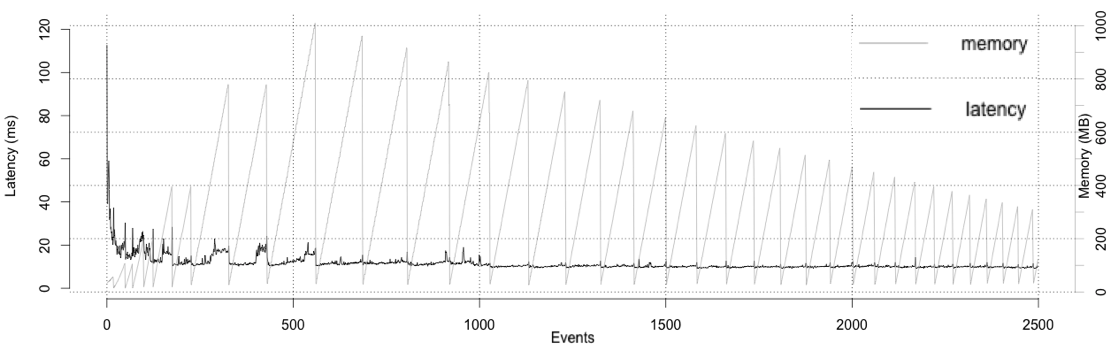
\includegraphics[width=0.70\linewidth]{images/comp-intra}
  }
\caption[\textsc{Analyser} Investigation Stack - Level 3 - Visual Comparison Examples]{\textsc{Analyser} Investigation Stack - Level 3 - Figure (a) shows a case of \textit{Inter Experiment} visual comparison of the memory usage while Figure (b) presents a case of \textit{Intra Experiment} comparison of latency and memory.}
  \label{fig:visual-comp}
\end{figure}